\documentclass[11pt, a4paper]{article}
\usepackage[utf8]{inputenc}
\usepackage{mathpazo} % Palatino font
\usepackage{lineno}
\usepackage{setspace}
\usepackage{caption}
\usepackage{graphicx, subfig}
\usepackage{graphicx, subcaption}
\usepackage{float} %so the graphs are not floating around after I put[H]
\usepackage[margin=2cm]{geometry}
\usepackage{indentfirst}
\usepackage{natbib} 
\bibliographystyle{agsm}
\usepackage{amsmath}
\usepackage{tabularx}
\usepackage{hyperref}
\usepackage[dvipsnames]{xcolor}
\hypersetup{
  colorlinks   = true, %Colours links instead of ugly boxes
  urlcolor     = blue, %Colour for external hyperlinks
  linkcolor    = black, %Colour of internal links
  citecolor   = black %Colour of citations
}

\newcommand{\reporttitle}{Changes in microbial community diversity along environmental gradients}
\newcommand{\reportauthor}{Chuxuan Ji}
\newcommand{\supervisor}{Samraat Pawar}
\newcommand{\degreetype}{Master of Research}
\newcommand{\multiref}[2]{\autoref{#1}-\ref{#2}} % from - to

\begin{document}
\begin{spacing}{1.5}
\input{./titlepage.tex}

\section*{Declaration}

I declare that the dissertation is my own work under the supervision of Dr. Samraat Pawar. All sources of information are appropriately referenced. No portion of the work referred to in the dissertation has been submitted in support of a degree or diploma or other qualification of this or any other university or other institute of learning. 

\clearpage

\section*{Abstract}
\addcontentsline{toc}{section}{Abstract}

Integrating information from global microbial research has been a massive obstacle to understanding microbial ecology. Identifying physical and chemical factors, such as temperature, pH or geography, associated with differences between different microbial communities will reveal the extent to which various types of environmental changes affect microbial diversity and will help us better understand microbial ecology and evolution. Here, I use the Environmental Microbiome Project global dataset to analyse bacterial diversity as a function of environmental gradients. Linear, polynomial regression and random forest models are used to fit the data to explore the environmental variables that have the most significant impact on bacterial diversity. I find that latitude probably performs best in predicting bacterial diversity in large-scale samples, while the temperature is a good choice in local samples. This study provides ideas of how microbial diversity varies with some fundamental environmental gradients. 

\clearpage

\tableofcontents 
\clearpage

\linenumbers
\renewcommand\thesection{\arabic{section}}
\section{Introduction}

One of ecology's main goals is to explain and predict biodiversity patterns \citep{mcgill2010towards}. Biodiversity is defined as the sum of all biological variation at all levels, from the genetic to the ecosystem \citep{purvis2000getting}. Microbes are some of the most abundant and diverse organisms globally, and bacteria are likely to make up the majority of biodiversity and a large proportion of biomass on Earth \citep{bar2018biomass}. However, the small size of microorganisms, their difficulty in cultivating, and the enormous complexity of microbial communities have led to much less research on microorganisms than on larger organisms. Metagenome analysis can reveal a lot about the composition and function of microbial communities, and it's become one of the significant points of microbial research \citep{mitchell2018ebi}. Microbes play an essential role in building ecosystems and the chemistry of the Earth's cycles \citep{azam1998microbial}. In the Earth's ecosystems, microorganisms regulate many ecosystem processes that are closely linked to climate through complex interactions and feedback mechanisms \citep{azam2007microbial, falkowski2008microbial} while playing a significant role in the carbon \citep{singh2010microorganisms} and nitrogen cycles \citep{kuypers2018microbial}. For instance, microbial respiration accounts for 50$\%$ of global respiration (about 60 billion tonnes of carbon released annually) \citep{hutchins2019climate}, and the world's terrestrial organisms emit about 119 billion tons of carbon annually, half of which comes from heterotrophic soil microorganisms \citep{reay2007greenhouse}. At the same time, heterotrophic bacteria dominate the global marine ${\rm N_{2}}$ fixation \citep{halm2012heterotrophic}. 

Microbial communities and climate interact and change each other \citep{hutchins2019climate}. To be specific, climate change, such as drought and warming, leads to a loss of microbial diversity and abundance, which can alter the multifunctionality of ecosystems so that it can have a moderating effect on climate \citep{delgado2017soil, delgado2016microbial}. Furthermore, microbial communities play an essential role in providing informative feedback on the environment. For instance, changes in marine microbes can well reflect the impact of global warming and ocean acidification \citep{boyd2018experimental}.  Moreover, the effects of climate change on microbes may reflect predictions for macroinvertebrates \citep{hotaling2019microbial}. Meanwhile, humans may harness microbial processes and thus better handle future climate change. Microbes' functions and feedback mechanisms in response to climate change can be reliably predicted by mastering long-term microbial datasets \citep{buttigieg2018marine, dore2009physical, saba2010challenges}. Microbes can also help mitigate anthropogenic climate change by enhancing agricultural productivity, producing biofuels, and vacuuming pollutants \citep{cavicchioli2019scientists}. The main factors that affect the diversity of different microbial communities are temperature, pH, environmental heterogeneity. By studying these factors, functional transitions and coping mechanisms of microbial communities in response to changes in niches and traits can be explored, which leads to a better understanding of microbial ecology and evolution \citep{lozupone2007global}. 

Temperature, precipitation and extreme climate changes due to global warming may cause microbial communities to adapt to new conditions or alter the geographical distribution of microbes \citep{leducq2014local}. Due to the change, factors affecting microbial communities may continue to change at regional and global scales. Global temperatures will increase by 0.25–0.32 °C per decade in the short-term future \citep{smith2018predicted}, while ocean pH is projected to decrease by a further 0.3–0.4 units by the end of the century \citep{caldeira2003anthropogenic, hurd2018current}. According to some research, modest temperature increases may have minimal impact on ecosystems in the short term, but permanent repercussions may ensue when it reaches a specific threshold \citep{scheffer2003catastrophic}. Since temperature is the fundamental driving factor for the metabolic rate of organisms according to the metabolic theory of ecology   \citep{brown2004toward}, and the temperature of the Earth's surface changes all the time, how temperature drives the metabolic rate of prokaryotes becomes particularly important \citep{thompson2017communal}. Changes in the rate of ecosystem processes ultimately depend on changes in the metabolic demands of individual organisms \citep{zhou2016temperature}. Meanwhile, experiments have shown that the diversity and composition of microbial functional genes respond rapidly to changes in temperature \citep{barria2013bacterial, wu2017alpine, xue2016tundra}. However, elevated temperature influences the stability of codon and anticodon interactions, as well as imposes selection restrictions on nucleic acid levels \citep{basak2005origin}. However, the results of studies on the relationship between temperature and microbial diversity at a global scale are varied and may show a linear increase, a linear decrease, a hump-shaped pattern, a trough-shaped pattern, or no pattern of diversity along a gradient \citep{garcia2013temperature, hendershot2017consistently, zhou2016temperature}. Thus, exploring the correlation between temperature and microbial diversity is crucial to understanding ecosystem functioning.

According to pH studies, ${\rm CO_{2}}$ levels could rise three to four times by the end of the 21st century compared to pre-industrial levels, which could raise the amount of dissolved ${\rm CO_{2}}$ on the water surface, changing the pH \citep{orr2005anthropogenic}. Controlling pH stabilisation at the cellular level is fundamental for cell function; therefore, pH control mechanisms are essential. Previous research on the relationship between environmental stability and the ability to adjust to future changes in environmental factors (such as pH) has suggested that ecological stability may limit adaptation capability \citep{somero2012physiology}. With global climate change, many habitats around the world (e.g., oceans and soils) are experiencing significant changes in pH \citep{caldeira2003anthropogenic, cavicchioli2019scientists}, which may affect community metabolism, growth, and reproduction through intracellular pH homeostasis \citep{melzner2009physiological}. This may lead to ecological impacts through, for example, the disappearance of specific species, which may affect local biodiversity and lead to disturbances in community composition. In turn, changes in pH conditions can lead to changes in oxygen consumption \citep{bunse2016response}, metabolism \citep{arnosti2011dynamics, grossart2006testing}, and food response \citep{piontek2010acidification} of the microbiome. The growth of microorganisms frequently causes substantial changes in surrounding pH, stimulating or impeding bacterial growth \citep{collins1987transfer, fu1999lactic, sole2000rapid}. In other words, pH influences a wide range of interactions within populations and between species \citep{ratzke2018modifying}. As ocean pH decreases, the energy required for bacterial cell maintenance increases rather than growth; the pH homeostatic mechanism takes up the majority of bacteria's transcriptional efforts, potentially affecting bacterial carbon cycling and energy fluxes in microbial food webs \citep{bunse2016response}. The most critical element in predicting the effect of global change factors (GCFs) on microbial alpha diversity is the pH of the soil \citep{zhou2020meta}. Investigating the impact of pH on microbial communities can help predict ecosystem changes and improve knowledge of climate change responses.

Here, I use data from the Earth Microbiome Project (EMP) \citep{thompson2017communal}, which includes plant, animal, non-saline and saline water bacterial samples, to explore the relationship between temperature, pH and latitudinal gradients and bacterial diversity, and hope to solve the question: \textit{What are the most important environmental drivers of change in the diversity of global bacterial communities?} Temperature is a fundamental driver of an organism's metabolic rate \citep{brown2004toward}, while pH stability at the cellular level is essential to cell function \citep{melzner2009physiological}, and they are both important drivers of microbial abundance \citep{cavicchioli2019scientists}. Meanwhile, environmental parameters closely related to latitude are considered to be critical ecological causes of latitudinal biodiversity patterns at large spatial/global scales \citep{mittelbach2007evolution, willig2013latitudinal}, such as climate stability, environmental stability, environmental predictability, seasonality and harshness \citep{kaufman1998structure, willig2013latitudinal}. Using latitude as a composite measure of these environmental parameters may be the better approach at large scales. Most studies of microbial diversity have been too limited spatially \citep{hanson2012beyond, martiny2006microbial, ramette2007biogeography, thompson2017communal}, so I explore the possible global patterns of microbial diversity and construct several models to provide some ideas to explain these patterns. 

\section{Material and Methods}

\subsection{Data}

All datasets analysed in this work have been previously published, and data are from the meta-analysis of the Earth Microbiome Project (EMP, \href{http://www.earthmicrobiome.org}{http://www.earthmicrobiome.org}) 16S Release 1. EMP includes the study of bacterial, archaeal, and eukaryotic microbial diversity \citep{thompson2017communal}. Only the bacterial portion of the entire database is taken for this analysis, and the QC-filtered subset used contains 96 studies and 23,828 samples (\href{https://zenodo.org/record/890000}{https://zenodo.org/record/890000}). This study uses a dataset that has been error-filtered and trimmed using Deblur software to the length of the shortest sequencing run (90 bp), and the resulting 90-bp Deblur BIOM table is used for all analyses. After excluding all samples with NA environmental data, this study analyses 23,820 samples belonging to 17 empo\_3 environmental taxa. Empo\_2 and empo\_3 category descriptions can be found at \href{http://www.earthmicrobiome.org/protocols-and-standards/empo}{http://www.earthmicrobiome.org/protocols-and-standards/empo}. Among them, Water (non-saline) (4915), soil (4279), and Animal distal gut (4158) account for the highest proportion in the dataset, and the dataset also include Aerosol (non-saline) (85) and Hypersaline (saline) (13) for this kind of classification with little data. When measuring the relationship between bacterial diversity and environmental variables, all samples that don't measure environmental variables (temperature and pH) are excluded because most of the data don't record temperature and pH. After the relationship is screened, 6977 samples from 11 empo\_3 environments are selected to explore the relationship between bacterial diversity and temperature, and 3986 samples from 10 empo\_3 environments are analyzed for the relationship between bacterial diversity and pH, and 23820 samples from 17 empo\_3 environments are analyzed for the relationship between bacterial diversity and latitude. In model fitting, 3066 samples from 8 empo\_3 environments with temperature, pH and latitude data are selected. 


\subsection{Biodiversity analysis}

This study considered the selection of various diversity indicators, such as observed richness, Chao1 estimated richness \citep{chao1984nonparametric}, Shannon-Wiener index \citep{hill2003using}, Simpson index and inverse Simpson index \citep{simpson1949measurement}. Ultimately, I chose alpha diversity based on observed richness, Chao1-estimated richness, and Shannon-Wiener index and formed a comparison of the three. In the results, the Chao1 index is mainly used as the display index in the main text.

\subsection{Model Fitting}

Regression models based on the normal distribution in linear models (LM) and polynomial regression models (PM) were used to fit the effects of environmental variables at different spatial scales on the microbial diversity index to predict the relationship between Chao1 Index and temperature, pH, and latitude. According to the Akaike information criterion (AIC) criterion, the "optimal model" was screened to determine the main driving factors, and the variance inflation factor (VIF) was used for collinearity diagnosis, and the variables with VIF \textless 10 were eliminated before refitting. 

At the same time, I used random forest (RF) models, which have the solid predictive ability not just for nonlinear data processing but also for datasets with many samples \citep{breiman2001random, cutler2007random}. Random forest models were utilised to investigate the impact of environmental factors and describe complicated relationships between environmental variables and bacterial diversity. I utilised a percentage increase in the MSE (Mean Squared Error) of a variable to measure the importance of these diversity indices: a higher MSE percent value indicates a more critical variable. The results could also be used to determine the value of each environmental variable, which can choose the factor that has the most significant effect on bacterial diversity.
 

\subsection{Statistical analyses}
All Statistical analyses and plots were run in R statistical software V4.1.1 and V3.6.3 \citep{team2013r} by using the packages vegan 2.5-7 \citep{oksanen2013package}, ggplot2 3.3.5 \citep{wickham2011ggplot2}, ggpubr 0.4.0 \citep{kassambara2020package}, dplyr 1.0.7 \citep{mailund2019manipulating}, lme4 1.1-27.1 \citep{bates2014fitting}, MASS 7.3-55 \citep{ripley2013package}, randomForest 4.6-11 \citep{rcolorbrewer2018package}, rfPermute 2.5 \citep{archer2016package}, A3 1.0.0 \citep{fortmann2015package}, car 3.0-11 \citep{fox2012package}, rockchalk 1.8.144 \citep{johnson2019package},.etc.

\section{Results}

\subsection{Relationships between bacterial diversity and environmental variables}

By observing the Chao1 index of the samples in the entire dataset, it can be observed that the samples of the four EMPO2 classifications have the most Chao1 index of 50-250, accounting for 14.89-45.33$\%$ of each classification (Figure \ref{fig:Chao_hist} A). At the same time, the number of non-saline samples increased significantly when the Chao1 index was around 2000, accounting for 11.66$\%$ of all non-saline samples (Figure \ref{fig:Chao_hist} B). In the non-saline samples, it can be observed that the Chao1 index of the soil and sediment samples is the largest when the Chao1 index is around 2000, while the Chao1 indices of the surface and water samples are the largest when the Chao1 indices are in the range of 50-250 (Figure \ref{fig:Chao_hist} B, Figure \ref{fig:Chao_hist3} A-D). In the saline samples, the number of water and surface samples is the largest when the Chao1 index is 50-250, while the Chao1 indices of the sediment sample are relatively average (Figure \ref{fig:Chao_hist} C, Figure \ref{fig:Chao_hist3} E-G). Among plant samples, Chao1 indices of rhizosphere samples are mostly greater than 1000, Chao1 indices of surface samples are primarily around 220, and Chao1 indices of corpus samples are mostly less than 100 (Figure \ref{fig:Chao_hist} D, Figure \ref{fig:Chao_hist3} H-J). The sample numbers of animal secretion, surface, corpus and distal gut are the largest when Chao1 index is around 75, 30, 25 and 125, respectively. When the Chao1 index is in the range of 200-950 and 0-400, the number of animal distal gut and proximal gut samples is average (Figure \ref{fig:Chao_hist} E, Figure \ref{fig:Chao_hist3} K-O).


\begin{figure}
    \centering
    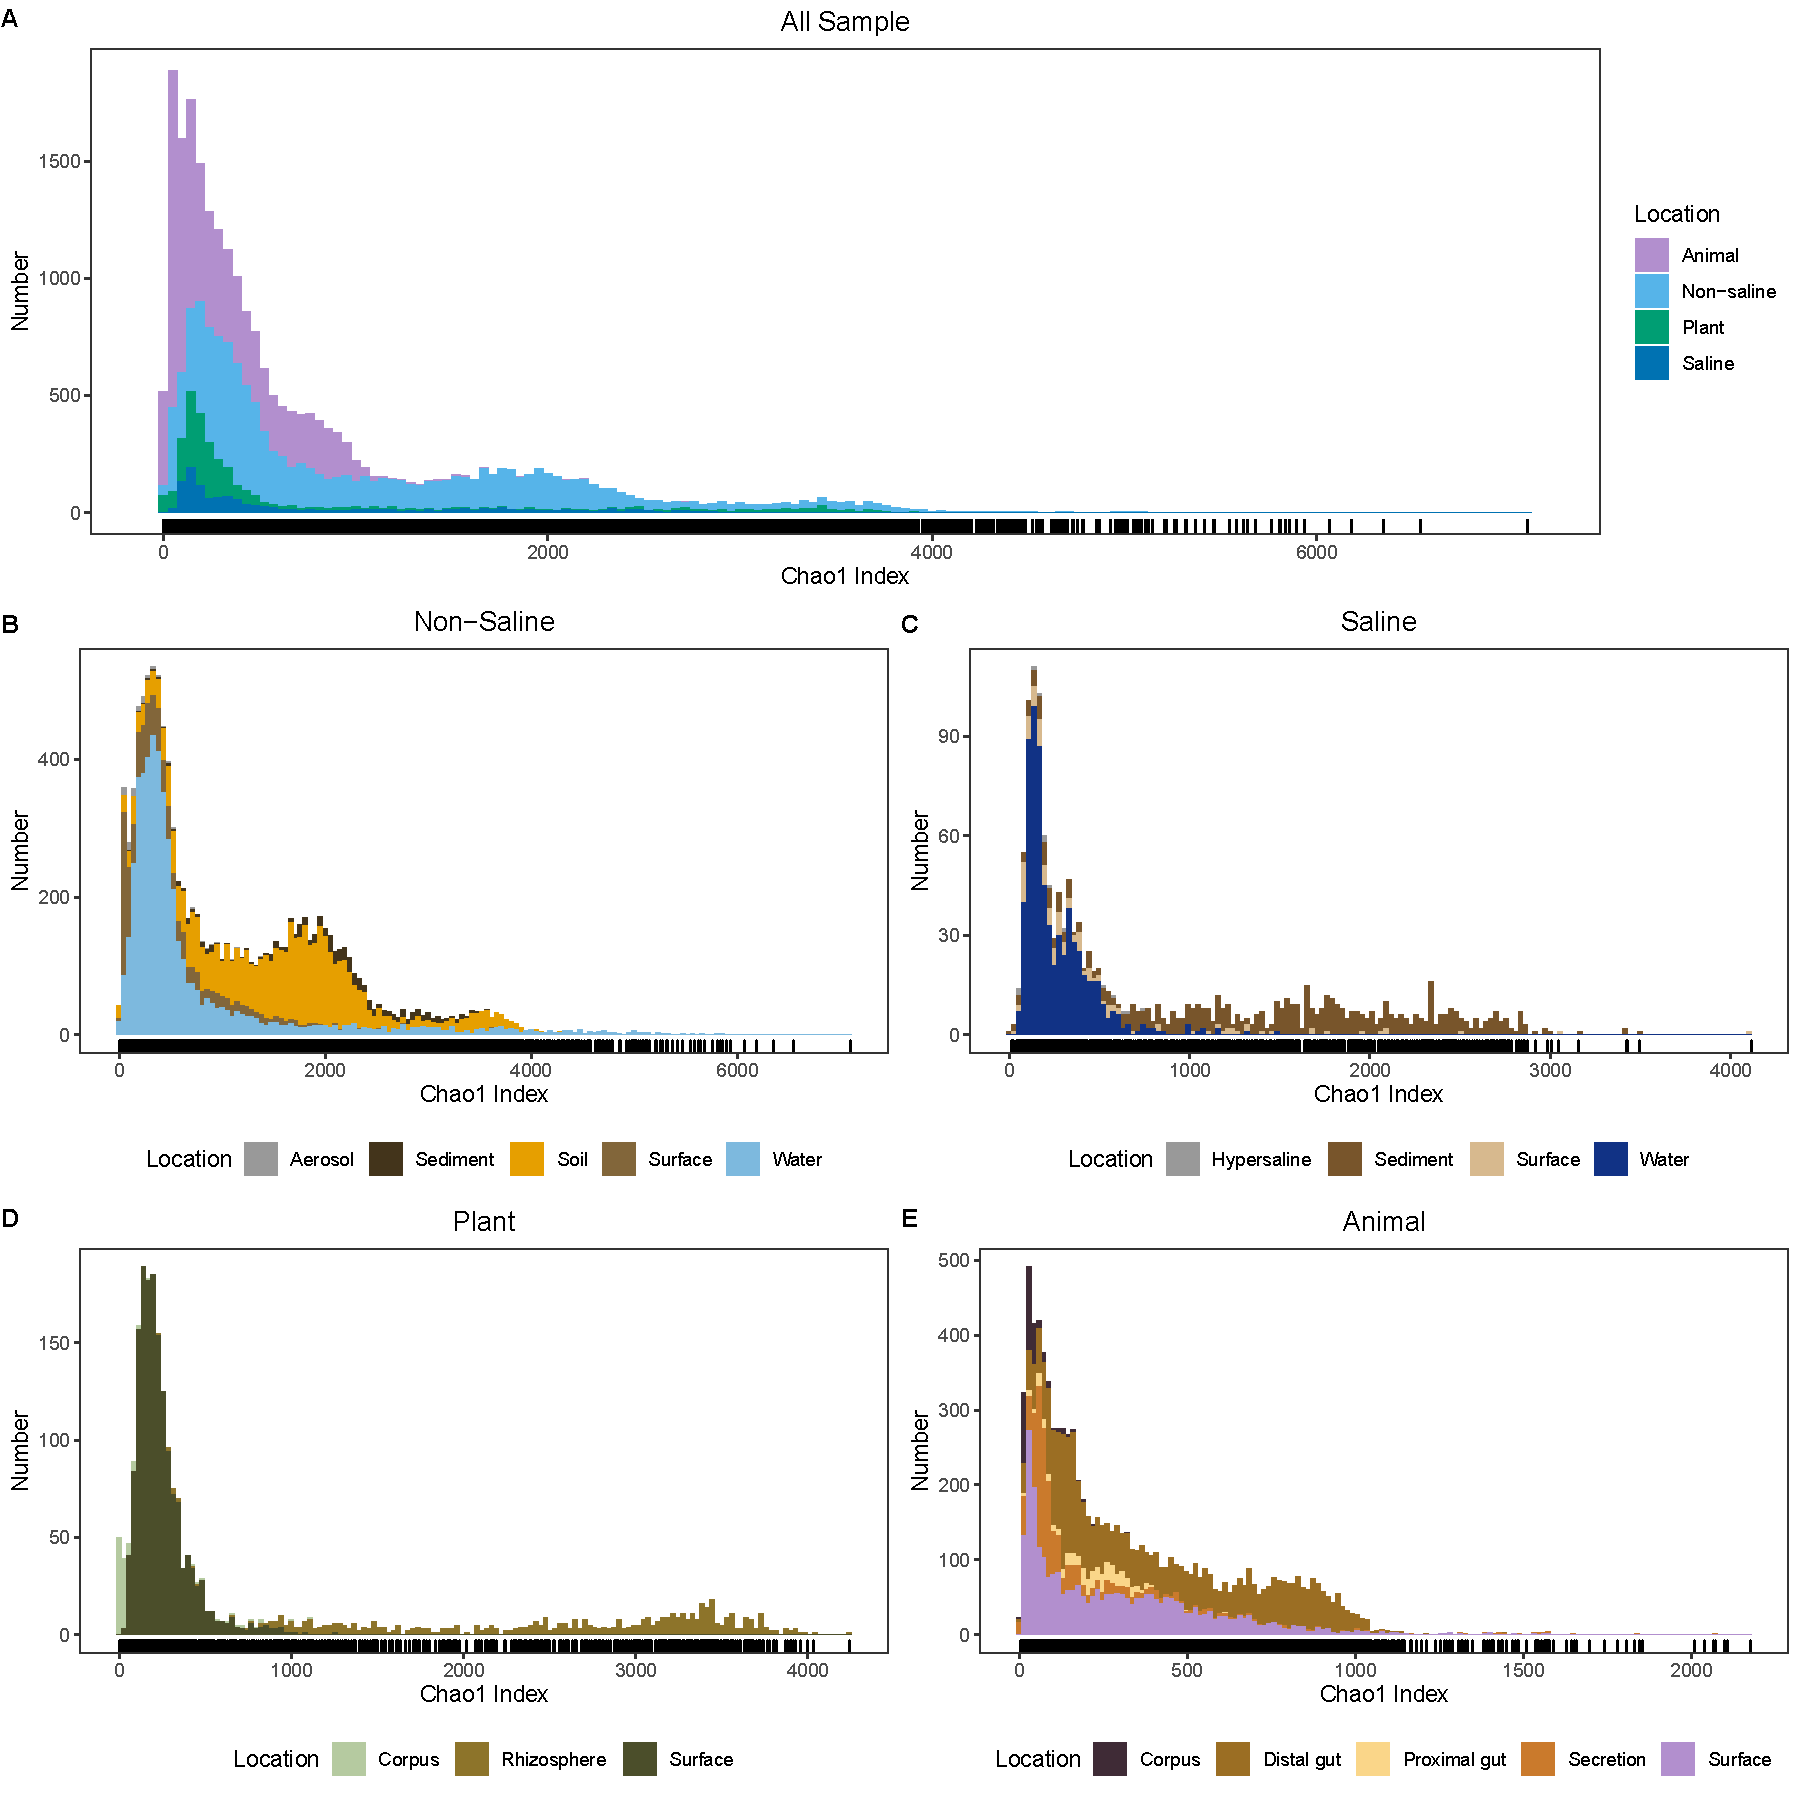
\includegraphics[scale=0.33]{./Figures/Chao_hist_empo2}
    \caption{\textbf{Distribution of Alpha Diversity in the whole dataset.} A: Distribution of Chao1 index values in the total dataset (23,820 samples, bin=150). B: Distribution of Chao1 index values for non-saline samples (11094 samples, bin=150). C: Distribution of Chao1 index values for saline samples (1373 samples, bin=150). D: Distribution of Chao1 index values for plant samples (2290 samples, bin=150). E: Distribution of Chao1 index values for animal samples (9071 samples, bin=150).}
    \label{fig:Chao_hist}
\end{figure}

When analysing the relationship between temperature and Chao1, it is found that the Chao1 index of bacteria is the highest at around 10 \textdegree C, which is also present in the non-saline and saline samples (Figure \ref{fig:Chao_T} A-C). Bacterial richness was highest in neutral environments in non-saline and saline samples (Figure \ref{fig:Chao_pH}). In the relationship between latitude and bacterial richness, the Chao1 indices are highest in the mid-latitude region in all samples (Figure \ref{fig:Chao_lati} A). In the EMPO2 classification, saline, plant, and animal samples all have the highest richness at mid-latitudes, while the richness of non-saline samples decreases with increasing latitude (Figure \ref{fig:Chao_lati} B-E). However, in the EMPO3 classification, it can be clearly seen that the Chao1 indices in the middle latitudes are the highest in almost all classifications (Figure  \ref{fig:Chao_lati3}).

\begin{figure}
    \centering
    \includegraphics[scale=0.33]{./Figures/Chao_T_empo2}
    \caption{\textbf{The relationship between Chao1 index and temperature.} A: Trend of Chao1 index with temperature for samples in the whole dataset. B: Trend of Chao1 index with temperature for non-saline samples. C: Trend of Chao1 index with temperature for saline samples. D: Trend of Chao1 index with temperature for plant samples.}
    \label{fig:Chao_T}
\end{figure}

\begin{figure}
    \centering
    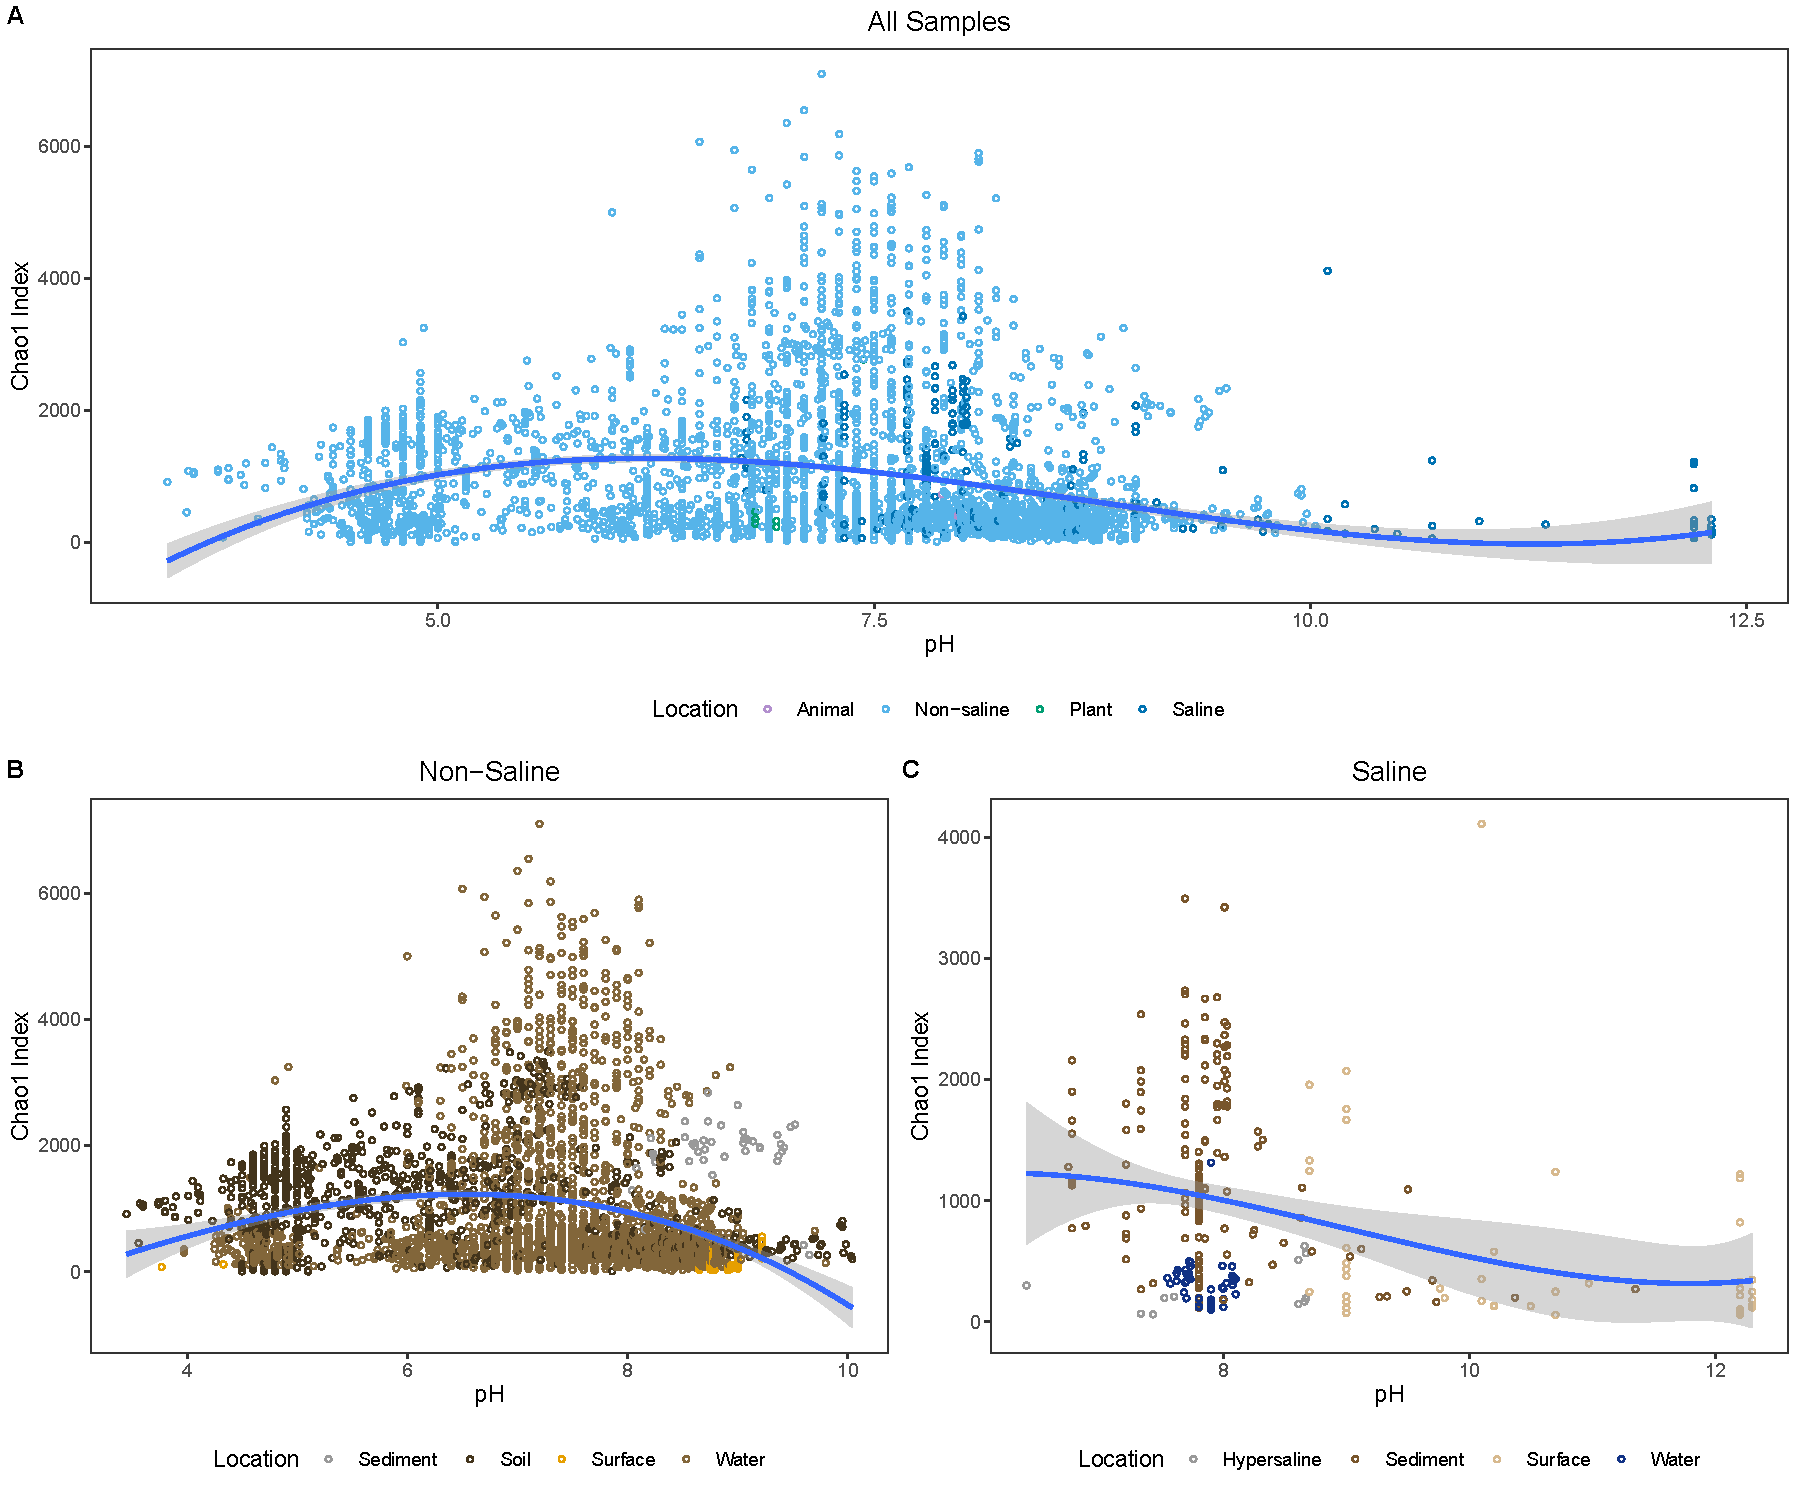
\includegraphics[scale=0.33]{./Figures/Chao_pH_empo2}
    \caption{\textbf{The relationship between Chao1 index and pH.} A: Trend of Chao1 index with pH for samples in the whole dataset. B: Trend of Chao1 index with pH for non-saline samples. C: Trend of Chao1 index with pH for saline samples.}
    \label{fig:Chao_pH}
\end{figure}

\begin{figure}
    \centering
    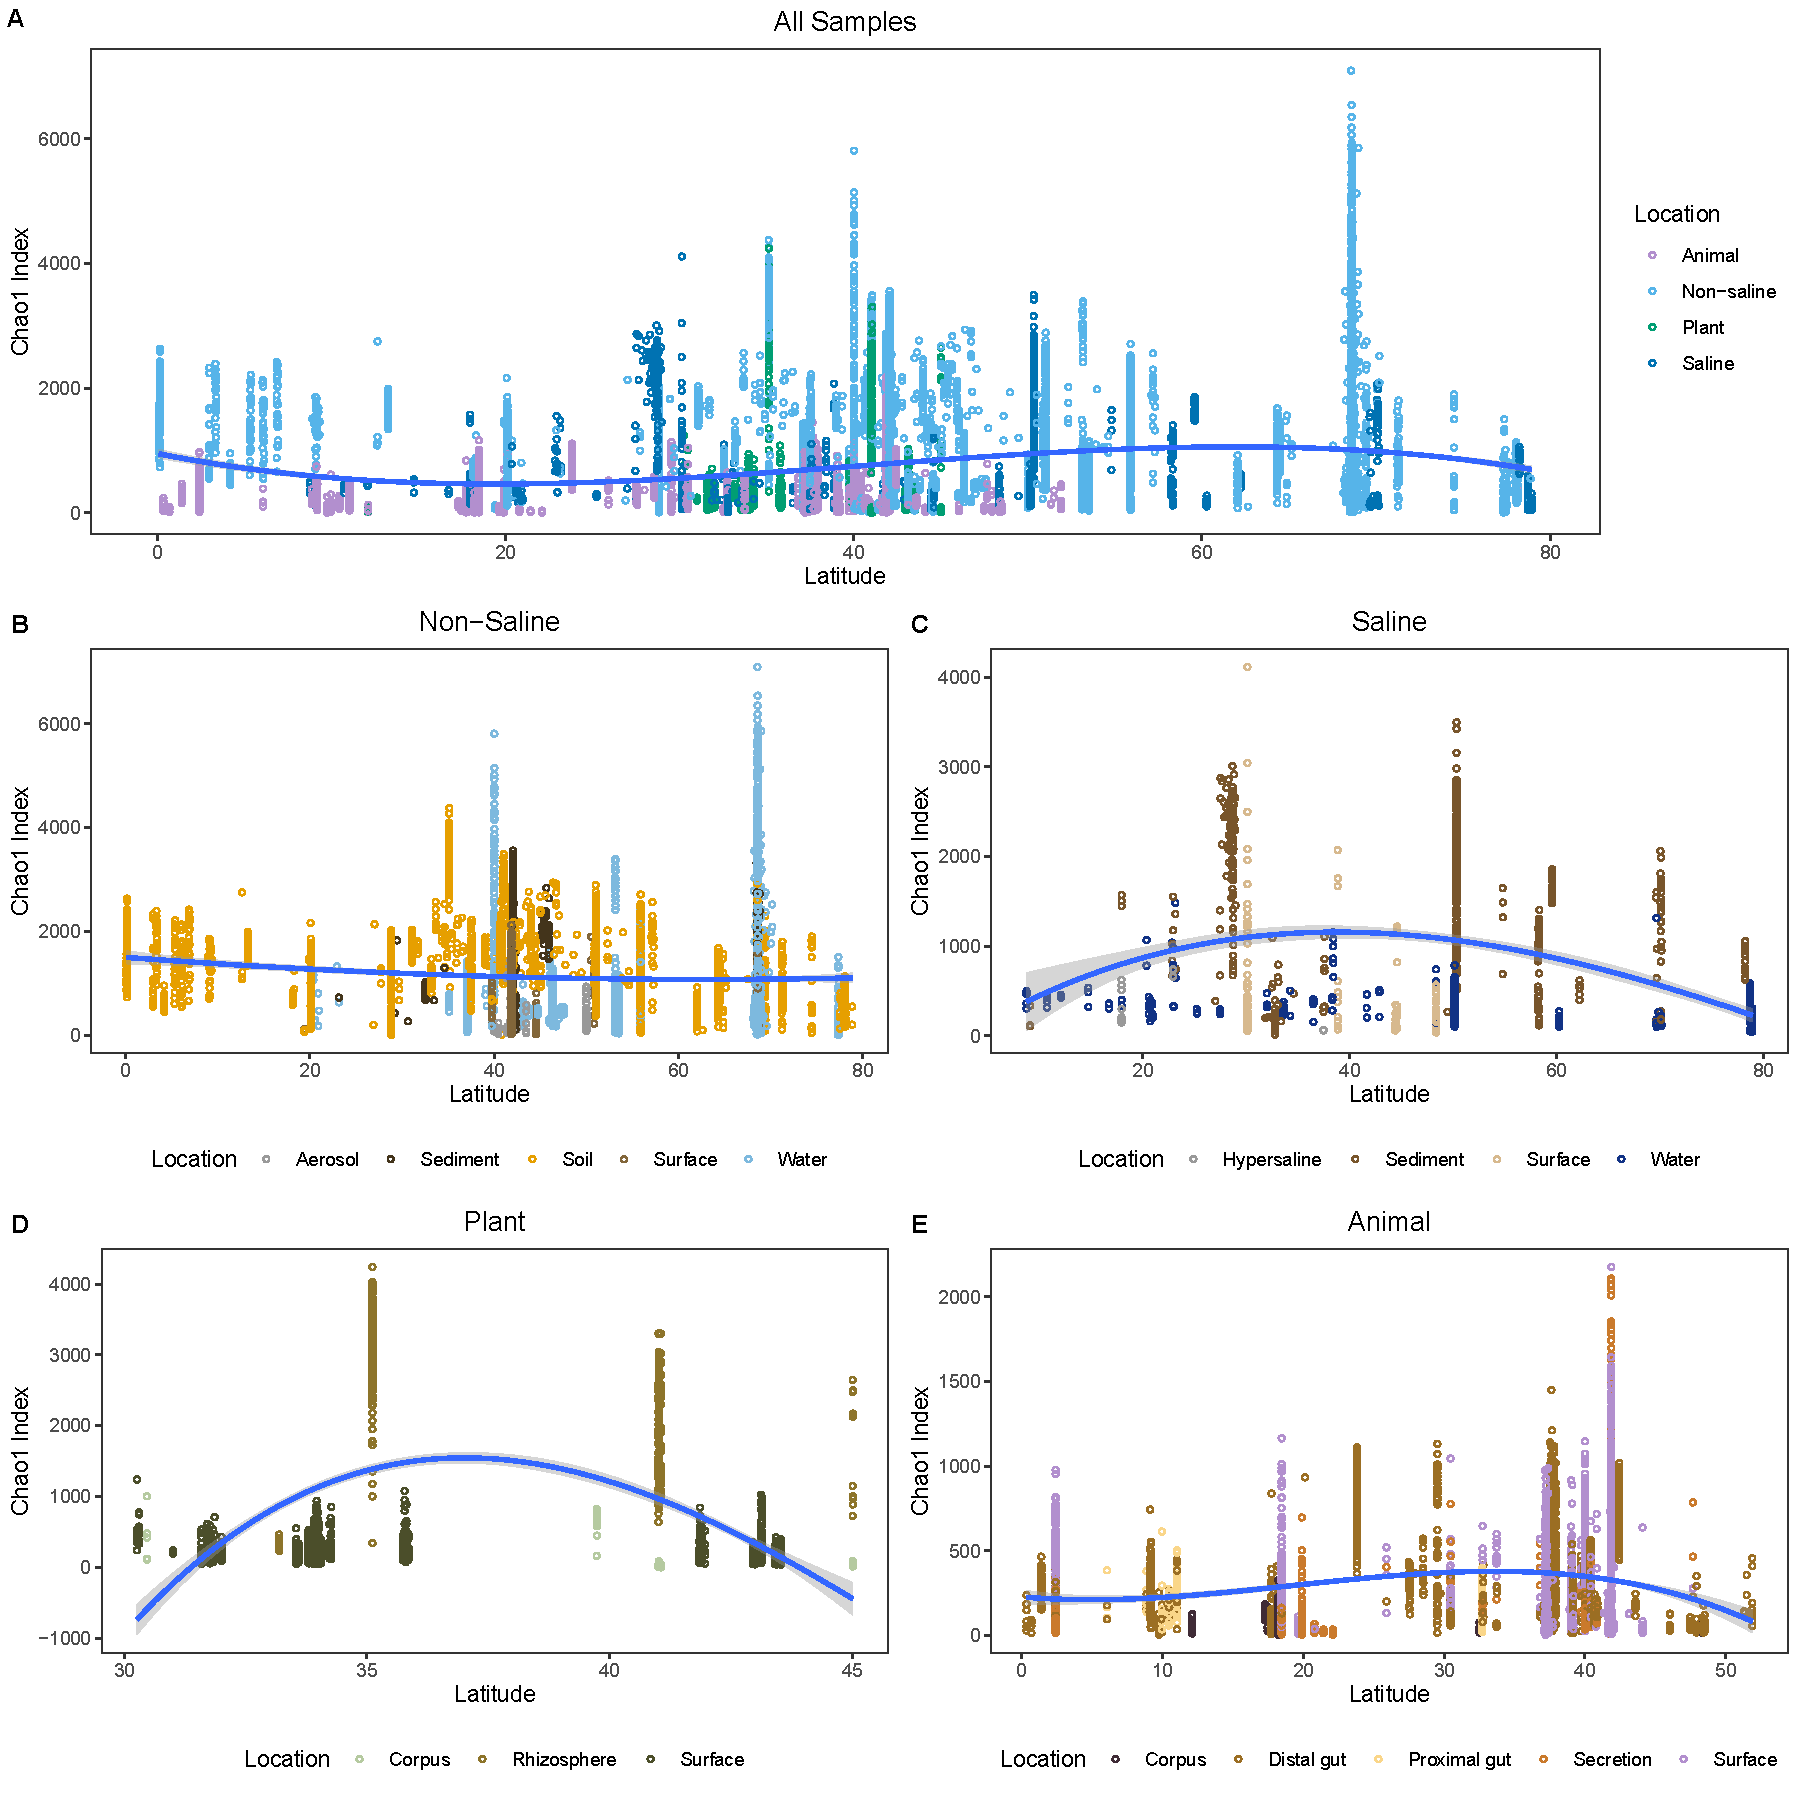
\includegraphics[scale=0.33]{./Figures/Chao_lati_empo2}
    \caption{\textbf{The relationship between Chao1 index and latitude.} A: Trend of Chao1 index with latitude for samples in the whole dataset. B: Trend of Chao1 index with latitude for non-saline samples. C: Trend of Chao1 index with latitude for saline samples. D: Trend of Chao1 index with latitude for plant samples. E: Trend of Chao1 index with latitude for animal samples.}
    \label{fig:Chao_lati}
\end{figure}

The above patterns are also almost similar in Observed OTUs and Shannon indices (\multiref{fig:OO_hist}{fig:Shan_lati3}).

\subsection{The effects of environmental variables on bacterial diversity}

After judging that bacterial diversity was not significantly collinear with temperature, pH, and latitude (Figure \ref{fig:Pairs}), I perform linear model, polynomial regression model, and random forest model fitting bacterial richness and environmental variables. Here, I measure the effects of temperature, pH, and latitude and their interactions on the three types of alpha diversity, These models show variance in the importance of environmental variables (Table \ref{tab:models}). Then, I compare linear and polynomial regression models and present the impact of a single environmental variable and two environmental variables on bacterial richness (Figure \ref{fig:Chao_simpleTpL}, \ref{fig:Chao_2EVs}, \multiref{fig:OO_simpleTpL}{fig:Shan_2EVs}).

\begin{table}
    \caption{R-square of the models between Chao1 index, observed OTUs and Shannon index and environmental variables}
    \centering
    \begin{tabular}{ |m{2cm}<{\centering}|m{4cm}<{\centering}|m{4cm}<{\centering}|m{4cm}<{\centering}|} 
    \hline
     $R^{2}$ & Chao1 (LM) & Chao1 (PM) & Chao1 (RF) \\
     \hline
    T*p*L & 0.1077 & 0.1306 & 0.4231 \\
    T*p & NULL & 0.07243 & 0.1709 \\
    T*L & 0.0959 & 0.1177 & 0.4563 \\
    p*L & 0.08393 & 0.1073 & 0.4536 \\
    T & 0.0316 & 0.04382 & 0.078 \\
    p & 0.002732 & 0.05292 & 0.1183 \\
    L & 0.08333 & 0.09948 & 0.491 \\
    \hline
    \hline
     $R^{2}$ & Shannon (LM) & Shannon (PM) & Shannon (RF) \\
     \hline
    T*p*L & 0.1498 & 0.2193 & 0.3859 \\
    T*p & 0.07004 & 0.1201 & 0.2352 \\
    T*L & 0.1376 & 0.1972 & 0.3891 \\
    p*L & 0.1098 & 0.1586 & 0.3834 \\
    T & 0.06943 & 0.081 & 0.0835 \\
    p & 0.002394 & 0.07006 & 0.1591 \\
    L & 0.108 & 0.1445 & 0.4049 \\
    \hline
    \hline
     $R^{2}$ & Observed OTUs (LM) & Observed OTUs (PM) & Observed OTUs (RF) \\
     \hline
    T*p*L & 0.09868 & 0.1271 & 0.4374 \\
    T*p & NULL & 0.0757 & 0.1794 \\
    T*L & 0.08696 & 0.1136 & 0.4699 \\
    p*L & 0.06803 & 0.0921 & 0.4561 \\
    T & 0.04028 & 0.05232 & 0.0832 \\
    p & 0.001798 & 0.04792 & 0.1155 \\
    L & 0.06739 & 0.08313 & 0.4963 \\
    \hline
    \end{tabular}    
    \label{tab:models}
\end{table}

\begin{figure}
    \centering
    \includegraphics[scale=0.33]{./Figures/Chao_LM_PM_simpleTpL}
    \caption{\textbf{Linear and polynomial regression models of Chao1 index with a single environmental variable.} A: Linear model of Chao1 index versus temperature. B: Linear model of Chao1 index versus pH. C: Linear model of Chao1 index versus latitude. D: Polynomial regression model of Chao1 index versus temperature. E: Polynomial regression model of Chao1 index versus pH. F: Polynomial regression model of Chao1 index versus latitude.}
    \label{fig:Chao_simpleTpL}
\end{figure}

\begin{figure}
    \centering
    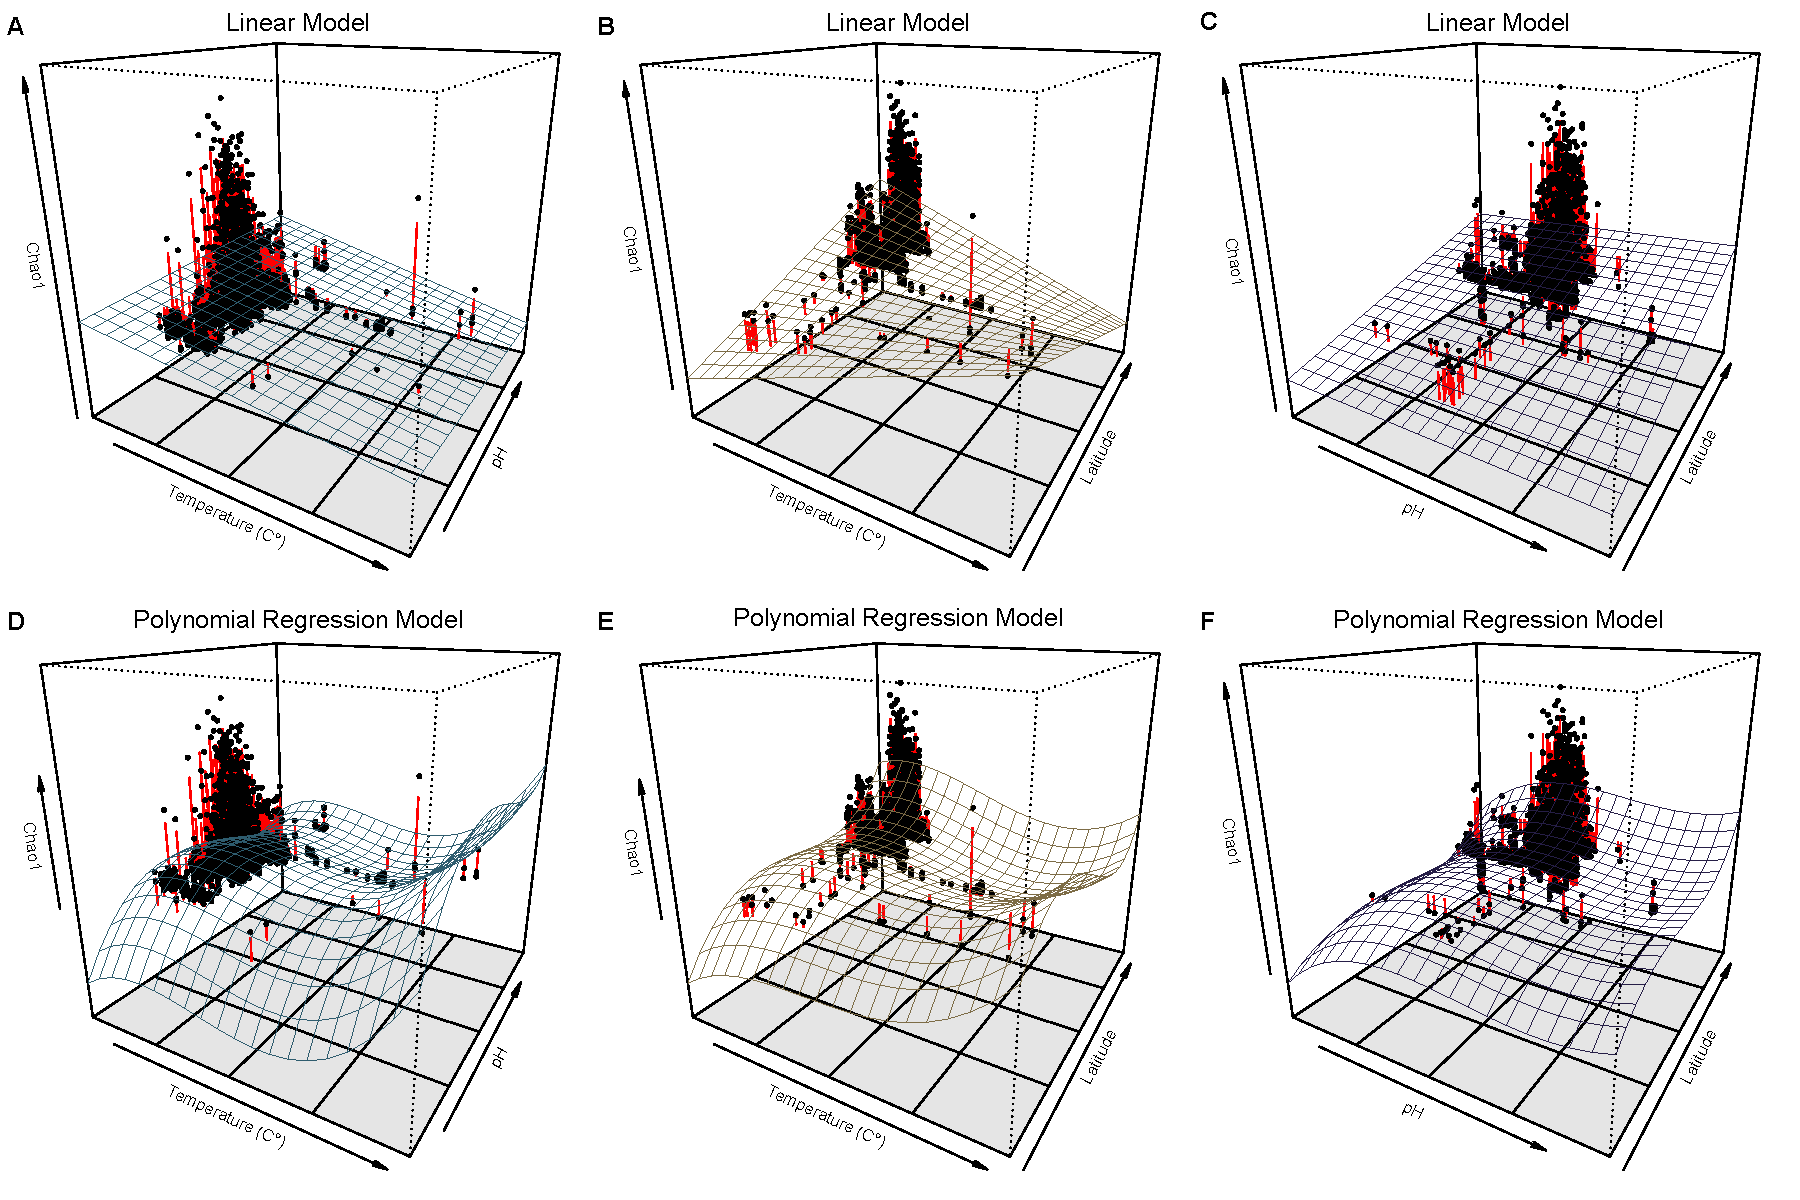
\includegraphics[scale=0.33]{./Figures/Chao_LM_PM_all_2EVs_3D}
    \caption{\textbf{Linear and polynomial regression models of Chao1 index with two environmental variables.} A: Linear model of Chao1 index versus temperature and pH. B: Linear model of Chao1 index versus temperature and latitude. C: Linear model of Chao1 index versus pH and latitude. D: Polynomial regression model of Chao1 index versus temperature and pH. E: Polynomial regression model of Chao1 index versus temperature and latitude. F: Polynomial regression model of Chao1 index versus pH and latitude.}
    \label{fig:Chao_2EVs}
\end{figure}

There is an interesting phenomenon among three kinds of models, whose results show that the variances of the latitude-dependent models are more significant than that of the models independent of it (Table \ref{tab:models}). The  most considerable model variance in the linear model is the effect of temperature, pH, and latitude (including interactions) on richness, while the pH one is the smallest. The Polynomial regression model performs better than the linear model, where the temperature, pH and latitude (including interactions) factor is still the most influential overall. At the same time, the worst performance is the diversity and temperature/pH model. The results of the random forest models show the best results. Among them, latitude explained 40.49-49.63$\%$ of the diversity models variances, followed by temperature and latitude, pH and latitude, and temperature, pH and latitude, while the temperature model had the most negligible variance (0.078-0.0835). 

To explore the relationship between bacterial diversity and environmental variables in specific environments, I select the three EMPO3 categories with the most significant number of samples in the dataset, namely non-saline water (2529), non-saline surface (195), and saline sediment (147). My EMPO3 models show a slight difference to the overall sample in predicting bacterial richness (Table \ref{tab:EMPO3models}). Both linear and polynomial regression models for the three EMPO3 environmental samples show that latitude-related factors are the most influential factors on the diversity index. In contrast, pH-related factors perform the worst in non-saline water and saline sediment samples. In saline sediment samples, only pH and latitude (including interactions) and latitude are linearly related to Shannon's exponent. In the linear and polynomial regression models of the non-saline surface, the performance of pH and latitude are not satisfactory. The fitting effect is generally better than the other two models in the random forest model. However, as the number of samples decreases, the fitting effect of the random forest model decreases. For example, in non-saline surface and saline sediment environments, it appears that the variances of some linear models and polynomial regression models are more significant than those of random forest models. Non-saline water samples are almost the same as the total samples. In the non-saline surface samples, the other environmental variables’ variances are not much different except for the latitude's more minor variance. All environmental variables in the saline sediment samples explain the diversity indices to a similar extent.

As the geographic scale gets smaller, latitude plays a smaller and smaller role. To this end, I explored samples from Yellowstone National Park (193), Großer Stechlinsee (1040), and Toolik Lake (1386) \citep{crump2012microbial} included in the EMP data, hoping to find the environmental factor that has the most significant impact on bacterial community diversity in local samples. All three kinds of models show almost the same results (Table \ref{tab:localmodels}); that is, the variances of the temperature models are basically more considerable than those of the pH models except for the local1 samples, and even in some models, the relationships between pH and diversity indices are not significant. In the local1 samples, the temperature and pH variances are not significantly different, which means that both variables significantly affect bacterial diversities.

\section{Discussion}

To study the impact of environmental variables on bacterial diversity in global samples, I selected three of the most easily measurable environmental factors, temperature, pH, and latitude, for diversity studies. My findings suggest that latitude may best predict bacterial diversity in large-scale range samples, while the temperature is highly recommended in local samples.  

The global pattern of microbial diversity is elusive, but understand the impact of different environmental factors on microbes and predict changes in microbial diversity across environmental gradients. The discovery of 16S rRNA genes in environmental samples has transformed our comprehension of microbial systematics and diversity, indicating how far we still have to go in identifying the wide assortment of bacteria on this planet \citep{hugenholtz1998impact, pace1997molecular, schloss2004status}. However, to date, integrating information from microbial research across the globe has been a massive obstacle to understanding microbial ecology. Identifying physical and chemical factors associated with differences between different microbial communities, such as temperature \citep{hicks2018temperature, kitidis2017seasonal}, pH \citep{delgado2019cross, fierer2006diversity}, or geography \citep{bates2013global, bik2012metagenetic, salazar2016global}, will reveal the extent to which various types of environmental changes affect microbial diversity and will help us better understand microbial ecology and evolution \citep{lozupone2007global, moran2015global, shoemaker2017macroecological}. 

Geographical patterns of bacterial diversity may help people better understand the prevalence of microbial community patterns and the mechanisms in organisms that respond to environmental changes \citep{fuhrman2008latitudinal}. My findings show that bacterial diversity peaks at mid-latitudes, a pattern that likely reflects the actual latitudinal diversity gradient from the equator to the poles. Meanwhile, latitude had the best effect on predicting bacterial diversity at the global scale. The latitudinal gradient is one of the oldest and most common biodiversity patterns worldwide, characterized by decreasing species richness from the tropics to the poles \citep{gaston1996biodiversity, gaston2000global, stevens1989latitudinal}. Contrary to previous beliefs, a growing body of biogeographic research indicates that whether animals, plants or microorganisms have peaks in biodiversity in temperate zones \citep{kerswell2006global, ladau2013global, lucifora2011global, phillips2019global, sato2021potential, tittensor2010global}. With global warming, climate change has led to previous changes in many ecosystem functions, with global mean surface temperature (GMST) increasing at a rate of 0.2° ± 0.1°C per decade \citep{change2007climate}. However, this has an enormous effect on tropical species \citep{antao2020temperature, colwell2008global, dillon2010global, pounds1999biological}, which have a narrower heat tolerance than temperate species, and which live at ambient temperatures very close to their physiological optimum \citep{deutsch2008impacts}. Warming could increase the abundance of many species that benefit from it and allow them to expand their geographic range \citep{chen2011rapid, hickling2006distributions, thomas2010climate}. Since most of the world's species are found in the tropics, warmer temperate regions at lower latitudes are likely to experience more extraordinary species richness and increases in abundance \citep{bates2014defining, tittensor2010global}. And this may be why bacterial diversity peaks at mid-latitudes. In previous studies, studies along latitudinal gradients have generally considered temperature change the driving variable as the factor most consistent with latitude change \citep{fierer2011microbes, gaston2000global}, however in my results, temperature and latitude are not closely related. According to current research, latitudinal diversity is influenced by five primary elements: sampling effort \citep{fierer2011microbes}, climate \citep{currie1991energy, hawkins2003energy}, spatial characteristics (such as area) \citep{rosenzweig_1995, terborgh1973notion}, biological interactions (such as competition and symbiosis), and evolutionary tendencies \citep{gaston2000global, willig2003latitudinal}, while factors such as climate stability, environmental stability, environmental predictability, seasonality and harshness, are all incorporated \citep{kaufman1998structure, willig2003latitudinal}. Latitude patterns are like any complex system \citep{10011263723}, so it's unlikely that any single variable will fully explain how species diversity occurs. Therefore, viewing latitude as an integrated mechanism of multiple factors may aplly to most biodiversity analyses \citep{gaston2000global, willig2003latitudinal}. 

Ecological metabolic theory suggests that temperature is a basic driver of biological metabolic rates \citep{brown2004toward}, which profoundly affects all life on Earth. Temperature controls the chemical reaction rates and pathways of organisms \citep{birgander2018responses, dacal2019soil,walker2018microbial}, and it affects the growth rate of microorganisms by affecting the thermal stability of proteins, thereby regulating biological pathways and mechanisms \citep{corkrey2012universality}. The diversity index peaked at around 10 \textdegree C in the overall sample. At the same time, the results from my models show that temperature is strongly associated with bacterial diversity in local samples. Even though the results show that the variance of the temperature model in the local1 sample is smaller than that of the pH model, the difference is not significant. However, many models could not fit pH and bacterial diversity index, and most models between diversity index and temperature show relevant results. Therefore, the temperature is an essential environmental predictor of bacterial diversity in local samples. 

My random forest models show promising results when fitting samples with larger sample sizes. My polynomial regression models show more apparent trends and fit no less well than the random forest models when judging small sample sizes. While feasible in the EMP dataset, the diversity gradients we observe necessarily reflect only a subset of the sample types in which the variable is measured, with the present difference of diverse and unmeasurable diversity of biotic or abiotic variables in different samples. The filtered datasets containing temperature and pH data were only one-eighth the size of the initial datasets. At the same time, the number of samples in each environment is not very average, which may lead to the existence of the pattern of some environments that dominate the pattern of the entire dataset. Due to the absence of other environmental variables in the dataset, it is difficult to measure the impact of other environmental variables on microbial diversity. For example, salinity may be the most important environmental factor affecting global microbial diversity \citep{lozupone2007global}; pH has the most critical influence on microorganisms in many environments \citep{bunse2016response, fierer2006diversity,fierer2011microbes}; the impact of climatic conditions and global change factors on microbial diversity has also received more and more attention \citep{drenovsky2010land, picazo2020climate, scherrer2010infra, zhou2020meta}. Understanding how these characteristics impact the worldwide distribution of bacteria might be crucial for humans to understand global biodiversity development and maintenance processes.

Significantly improving the understanding of global microbial biodiversity is one of the most important goals of ecologists and biogeographers. These data suggest that latitude may be the most important environmental variable affecting bacterial diversity, and that bacterial diversity peaks at mid-latitudes. In local samples, the temperature is most strongly associated with bacterial diversity. While these data do not fully cover all environmental variables, given that many environments are more difficult to measure other than temperature, pH and geography, this study provides insights into how microbial diversity varies with some fundamental environmental gradients some ideas.

\section*{Code Availability}
\addcontentsline{toc}{section}{Code Availability}

The R code for models and analysis in this study is availible at the \href{https://github.com/ChuxuanJi/EECProject1}{\color{blue}{\underline{EEC MRes Winter Project}}} repository.

\section*{Acknowledgement}
\addcontentsline{toc}{section}{Acknowledgement}

I would like to express my greatest gratitude to Dr. Samraat Pawar for all his support and supervision throughout the entire project, even after his sabbatical started. I'm also sincerely grateful for all the inspiring ideas and thoughts Danica Duan (PhD candidate) and Dr. Tom Clegg provided throughout my project. And thank all three of them for providing feedback on my drafting thesis. I am very grateful to my parents, family and good friends for their great support and encouragement, and I am also very grateful to my girlfriend Xu Lan for her company across the ocean. In the end, I am also very grateful that I can continue to work hard in the direction I like. Every late night in front of the computer is an improvement for myself, and I hope that I can keep this spirit forever. 

\addcontentsline{toc}{section}{References}
\bibliographystyle{agsm}
\bibliography{thesis}
\clearpage


\begin{document}
\renewcommand{\thefigure}{SI.\arabic{figure}}
\setcounter{figure}{0}

\renewcommand{\thetable}{SI.\arabic{table}}
\setcounter{table}{0}

\section*{Supplementary Information}\label{sec:SI}

\addcontentsline{toc}{section}{Supplementary Information}
\addtocontents{toc}{\setcounter{tocdepth}{-10}}
\renewcommand{\thesubsection}{SI.\arabic{subsection}}
\setcounter{subsection}{0}


\subsection{Shannon Index and Observed OTUs plot}



\begin{figure}[H]
    \centering
    \includegraphics[scale=0.33]{./Figures/Chao_hist_empo3}
    \caption{\textbf{Distribution of Alpha Diversity in the empo\_3 samples.} A: Distribution of Chao1 index values for soil samples (4279 samples). B: Distribution of Chao1 index values for non-saline sediment samples (544 samples). C: Distribution of Chao1 index values for non-saline surface samples (1271 samples). D: Distribution of Chao1 index values for non-saline water samples (4915 samples). E: Distribution of Chao1 index values for saline sediment samples (559 samples). F: Distribution of Chao1 index values for saline surface samples (117 samples). G: Distribution of Chao1 index values for saline water samples (684 samples). H: Distribution of Chao1 index values for plant rhizosphere samples (554 samples). I: Distribution of Chao1 index values for plant surface samples (1611 samples). J: Distribution of Chao1 index values for plant corpus samples (125 samples). K: Distribution of Chao1 index values for animal secretion samples (1257 samples). L: Distribution of Chao1 index values for animal surface samples (2961 samples). M: Distribution of Chao1 index values for animal corpus samples (328 samples). N: Distribution of Chao1 index values for animal distal gut samples (4158 samples). O: Distribution of Chao1 index values for animal proximal gut samples (367 samples).}
    \label{fig:Chao_hist3}
\end{figure}

\begin{figure}[H]
    \centering
    \includegraphics[scale=0.33]{./Figures/Chao_lati_empo3}
    \caption{\textbf{The relationship between Chao1 index and latitude.} A: Trend of Chao1 index with latitude for soil samples. B: Trend of Chao1 index with latitude for non-saline water (water and sediment) samples. C: Trend of Chao1 index with latitude for saline water (water and sediment) samples. D: Trend of Chao1 index with latitude for non-saline sediment samples. E: Trend of Chao1 index with latitude for non-saline surface samples. F: Trend of Chao1 index with latitude for non-saline water samples. G: Trend of Chao1 index with latitude for saline sediment samples. H: Trend of Chao1 index with latitude for saline surface samples. I: Trend of Chao1 index with latitude for saline water samples. J: Trend of Chao1 index with latitude for animal surface samples. K: Trend of Chao1 index with latitude for plant surface samples. L: Trend of Chao1 index with latitude for plant rhizosphere samples.}
    \label{fig:Chao_lati3}
\end{figure}

\begin{figure}[H]
    \centering
    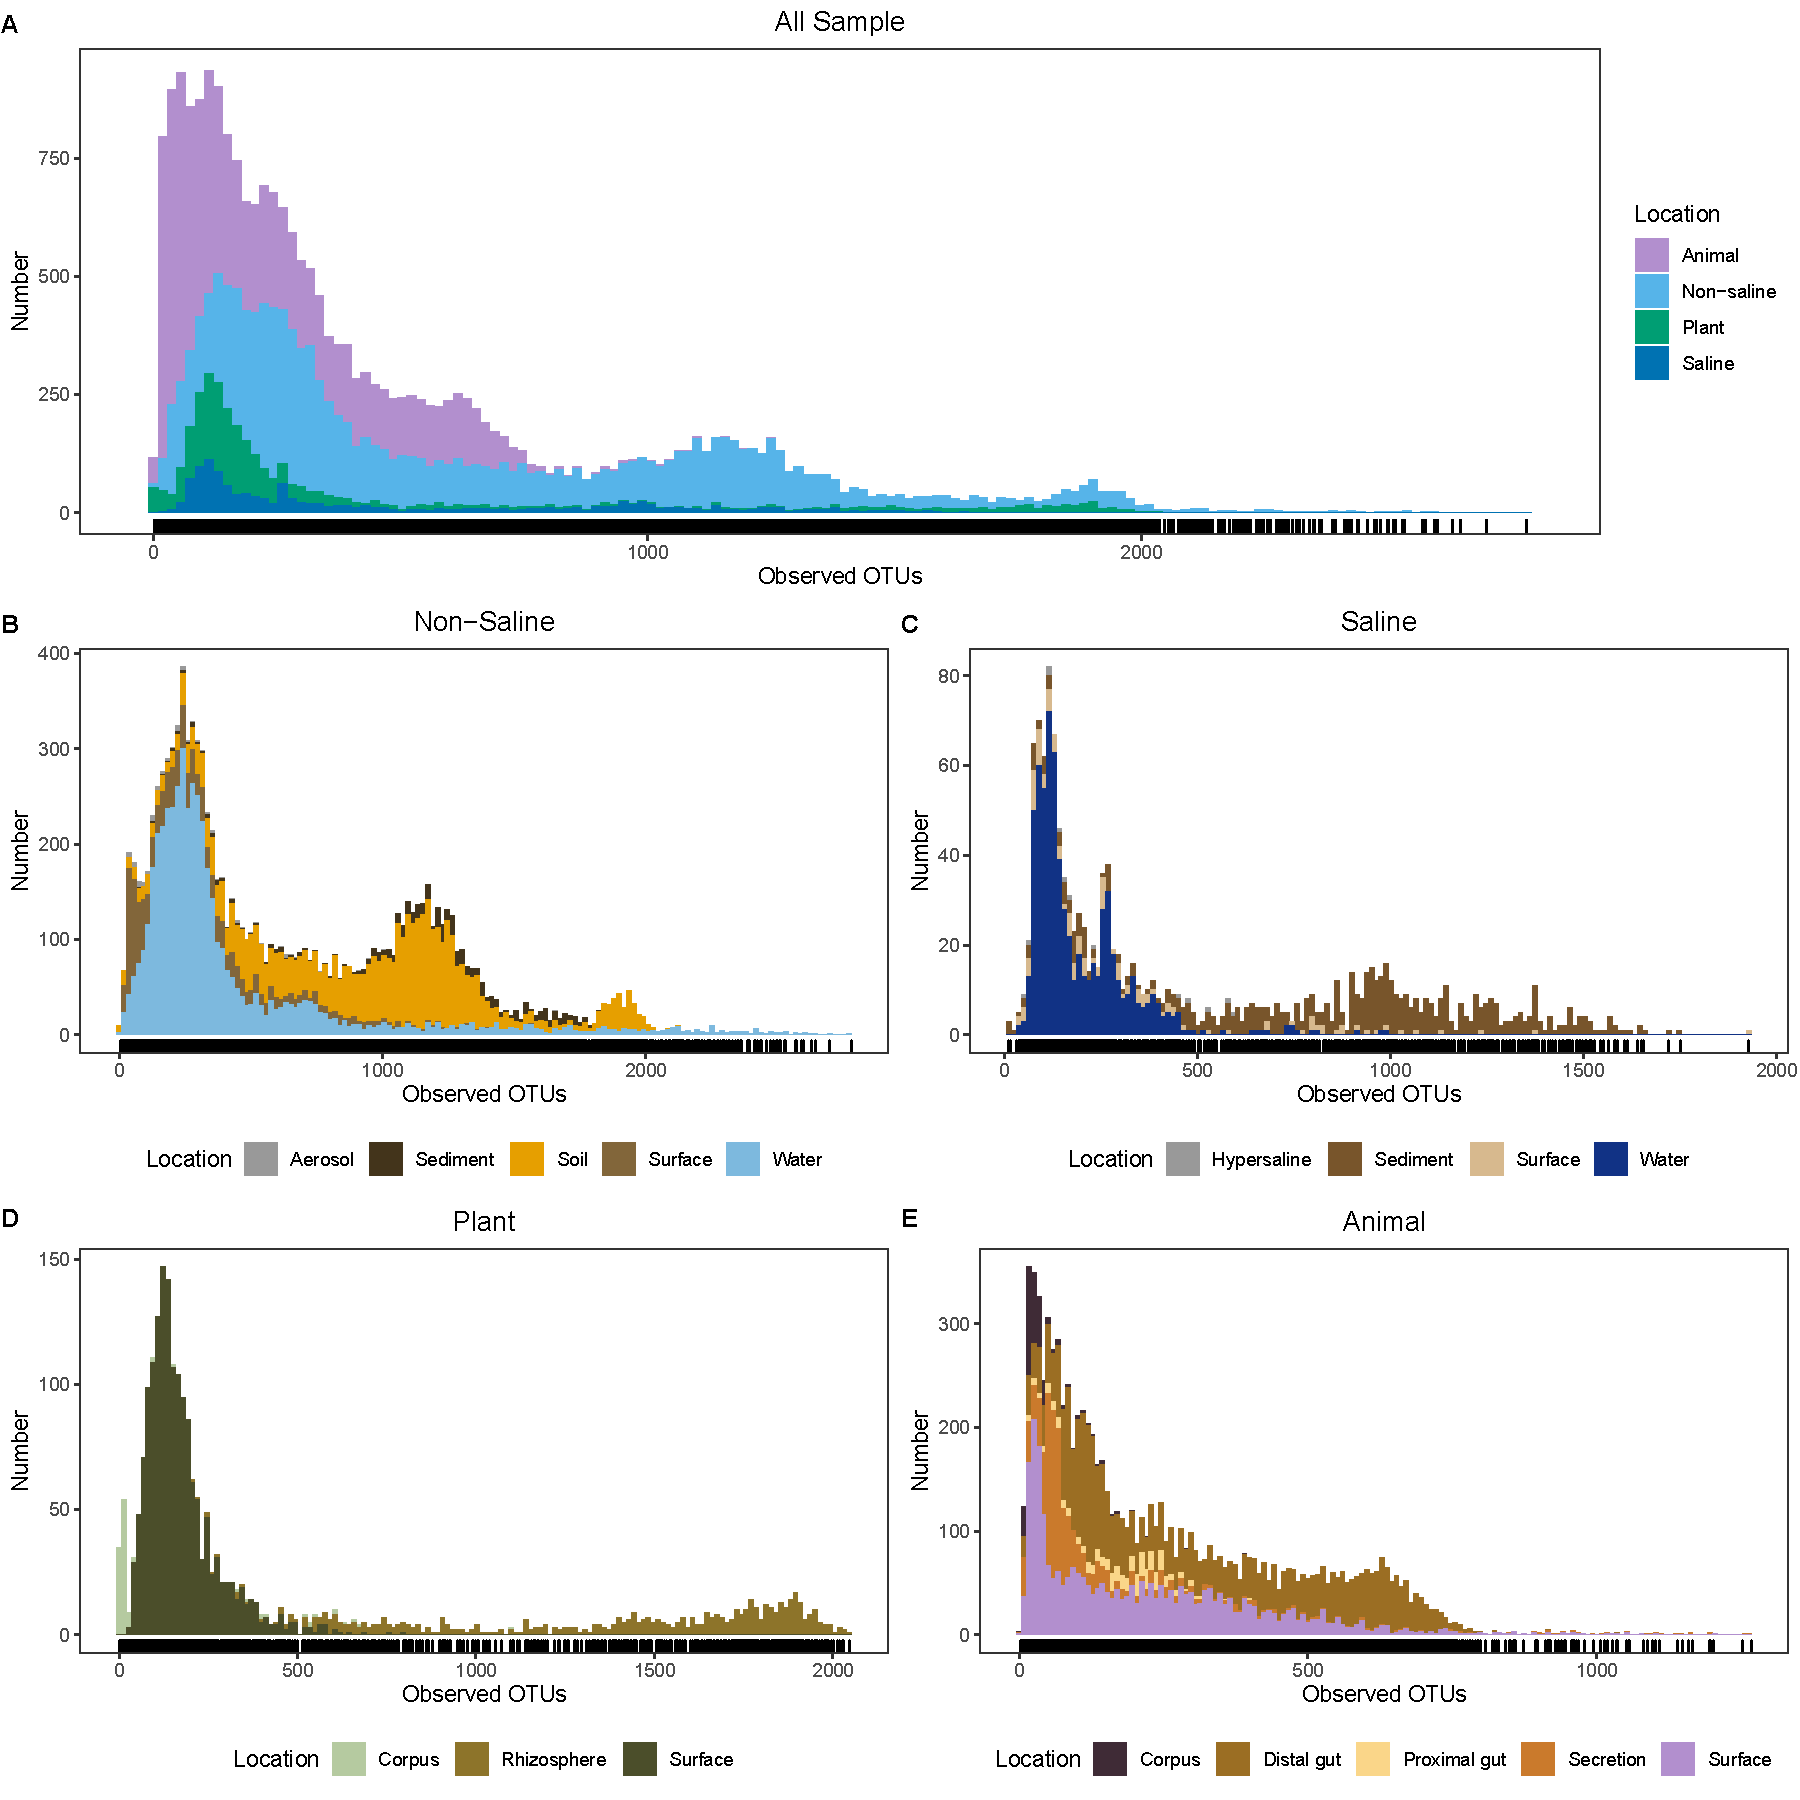
\includegraphics[scale=0.33]{./Figures/OO_hist_empo2}
    \caption{\textbf{Distribution of Observed OTUs in the whole dataset.} A: Distribution of Observed OTUs in the total dataset (23,820 samples, bin=150). B: Distribution of Observed OTUs for non-saline samples (11094 samples, bin=150). C: Distribution of Observed OTUs for saline samples (1373 samples, bin=150). D: Distribution of Observed OTUs for plant samples (2290 samples, bin=150). E: Distribution of Observed OTUs for animal samples (9071 samples, bin=150).}
    \label{fig:OO_hist}
\end{figure}

\begin{figure}[H]
    \centering
    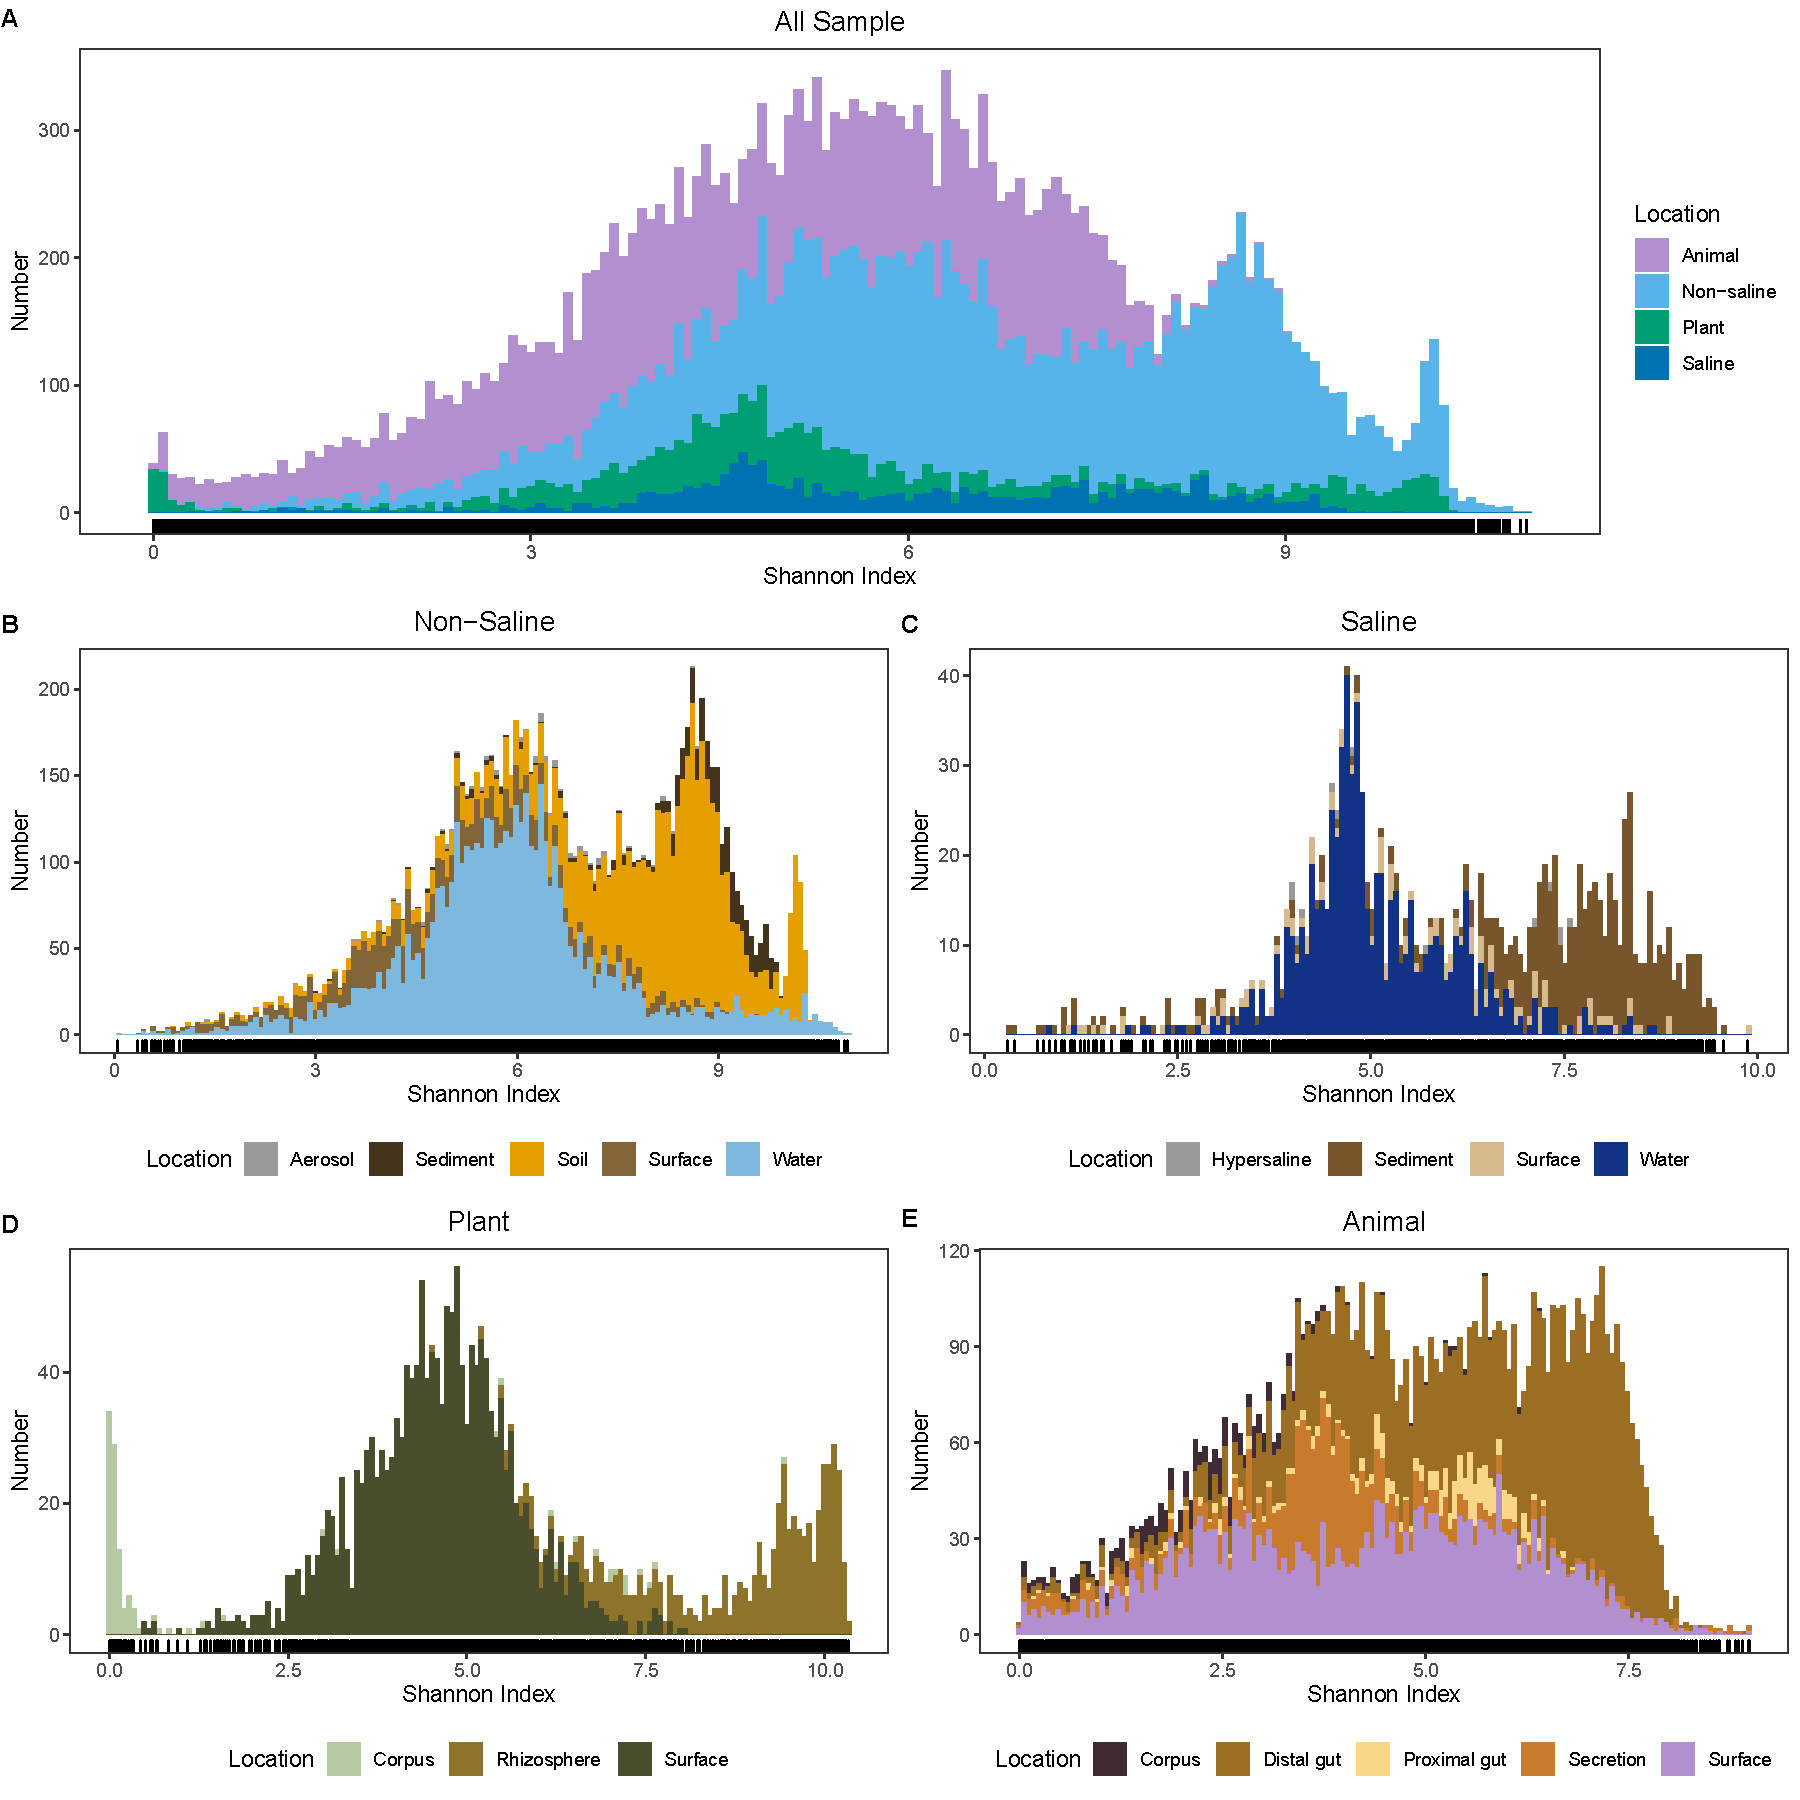
\includegraphics[scale=0.33]{./Figures/Shan_hist_empo2}
    \caption{\textbf{Distribution of Shannon index in the whole dataset.} A: Distribution of Shannon index values in the total dataset (23,820 samples, bin=150). B: Distribution of Shannon index values for non-saline samples (11094 samples, bin=150). C: Distribution of Shannon index values for saline samples (1373 samples, bin=150). D: Distribution of Shannon index values for plant samples (2290 samples, bin=150). E: Distribution of Shannon index values for animal samples (9071 samples, bin=150).}
    \label{fig:Shan_hist}
\end{figure}

\begin{figure}[H]
    \centering
    \includegraphics[scale=0.33]{./Figures/OO_hist_empo3}
    \caption{\textbf{Distribution of observed OTUs in the empo\_3 samples.} A: Distribution of observed OTUs for soil samples (4279 samples). B: Distribution of observed OTUs for non-saline sediment samples (544 samples). C: Distribution of observed OTUs for non-saline surface samples (1271 samples). D: Distribution of observed OTUs for non-saline water samples (4915 samples). E: Distribution of observed OTUs for saline sediment samples (559 samples). F: Distribution of observed OTUs for saline surface samples (117 samples). G: Distribution of observed OTUs for saline water samples (684 samples). H: Distribution of observed OTUs for plant rhizosphere samples (554 samples). I: Distribution of observed OTUs for plant surface samples (1611 samples). J: Distribution of observed OTUs for plant corpus samples (125 samples). K: Distribution of observed OTUs for animal secretion samples (1257 samples). L: Distribution of observed OTUs for animal surface samples (2961 samples). M: Distribution of observed OTUs for animal corpus samples (328 samples). N: Distribution of observed OTUs for animal distal gut samples (4158 samples). O: Distribution of observed OTUs for animal proximal gut samples (367 samples).}
    \label{fig:OO_hist3}
\end{figure}

\begin{figure}[H]
    \centering
    \includegraphics[scale=0.33]{./Figures/Shan_hist_empo3}
    \caption{\textbf{Distribution of Shannon index in the empo\_3 samples.} A: Distribution of Shannon index values for soil samples (4279 samples). B: Distribution of Shannon index values for non-saline sediment samples (544 samples). C: Distribution of Shannon index values for non-saline surface samples (1271 samples). D: Distribution of Shannon index values for non-saline water samples (4915 samples). E: Distribution of Shannon index values for saline sediment samples (559 samples). F: Distribution of Shannon index values for saline surface samples (117 samples). G: Distribution of Shannon index values for saline water samples (684 samples). H: Distribution of Shannon index values for plant rhizosphere samples (554 samples). I: Distribution of Shannon index values for plant surface samples (1611 samples). J: Distribution of Shannon index values for plant corpus samples (125 samples). K: Distribution of Shannon index values for animal secretion samples (1257 samples). L: Distribution of Shannon index values for animal surface samples (2961 samples). M: Distribution of Shannon index values for animal corpus samples (328 samples). N: Distribution of Shannon index values for animal distal gut samples (4158 samples). O: Distribution of Shannon index values for animal proximal gut samples (367 samples).}
    \label{fig:Shan_hist3}
\end{figure}

\begin{figure}[H]
    \centering
    \includegraphics[scale=0.33]{./Figures/OO_T_empo2}
    \caption{\textbf{The relationship between observed OTUs and temperature.} A: Trend of observed OTUs with temperature for samples in the whole dataset. B: Trend of observed OTUs with temperature for non-saline samples. C: Trend of observed OTUs with temperature for saline samples. D: Trend of observed OTUs with temperature for plant samples.}
    \label{fig:OO_T}
\end{figure}

\begin{figure}[H]
    \centering
    \includegraphics[scale=0.33]{./Figures/Shan_T_empo2}
    \caption{\textbf{The relationship between Shannon index and temperature.} A: Trend of Shannon index with temperature for samples in the whole dataset. B: Trend of Shannon index with temperature for non-saline samples. C: Trend of Shannon index with temperature for saline samples. D: Trend of Shannon index with temperature for plant samples.}
    \label{fig:Shan_T}
\end{figure}


\begin{figure}[H]
    \centering
    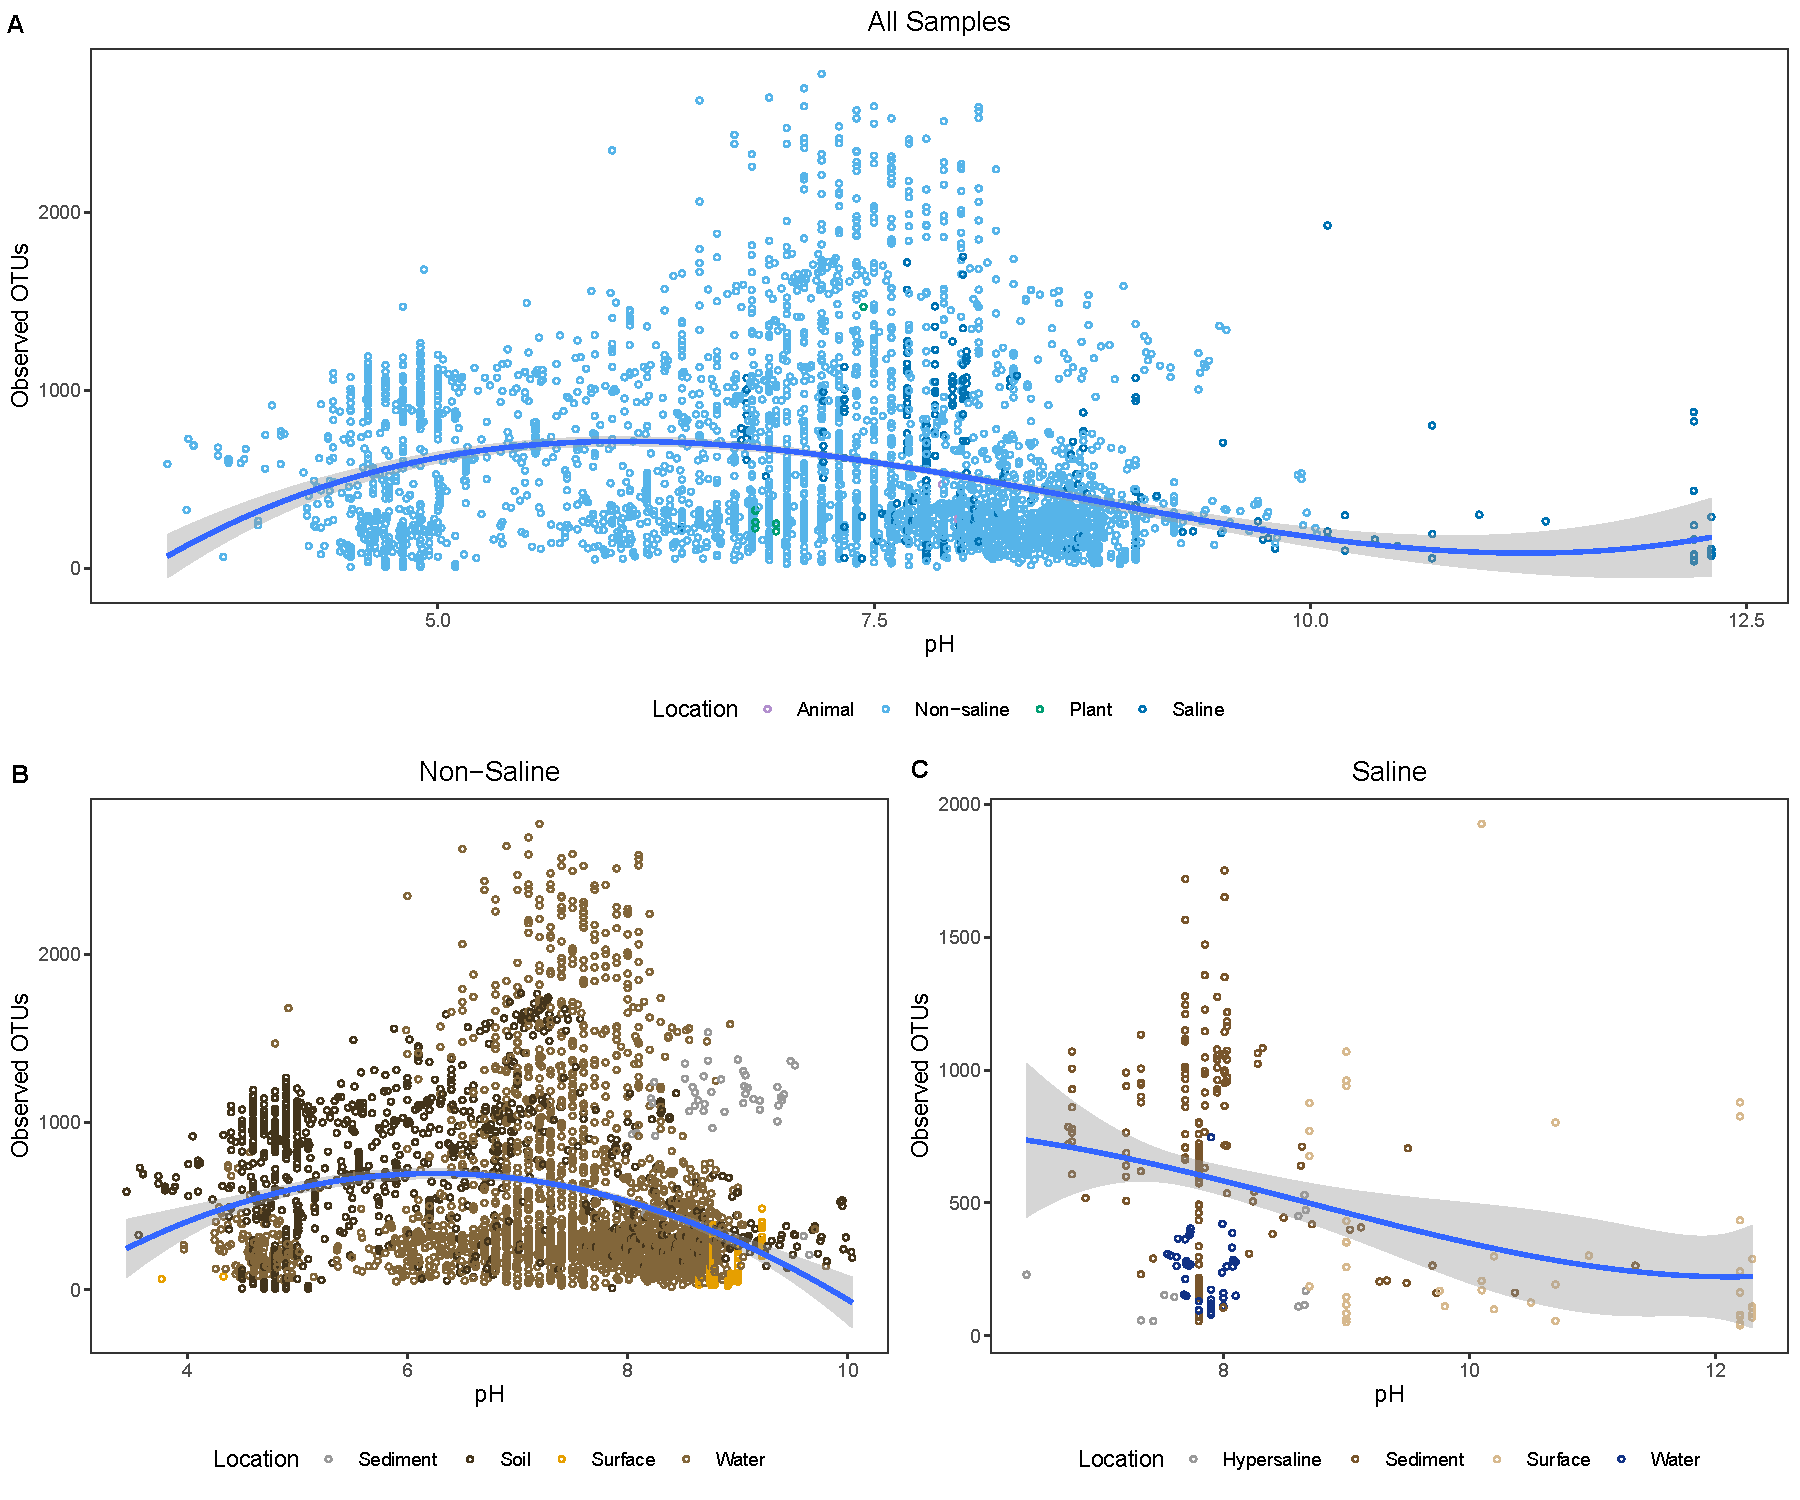
\includegraphics[scale=0.33]{./Figures/OO_pH_empo2}
    \caption{\textbf{The relationship between observed OTUs and pH.} A: Trend of observed OTUs with pH for samples in the whole dataset. B: Trend of observed OTUs with pH for non-saline samples. C: Trend of observed OTUs with pH for saline samples.}
    \label{fig:OO_pH}
\end{figure}

\begin{figure}[H]
    \centering
    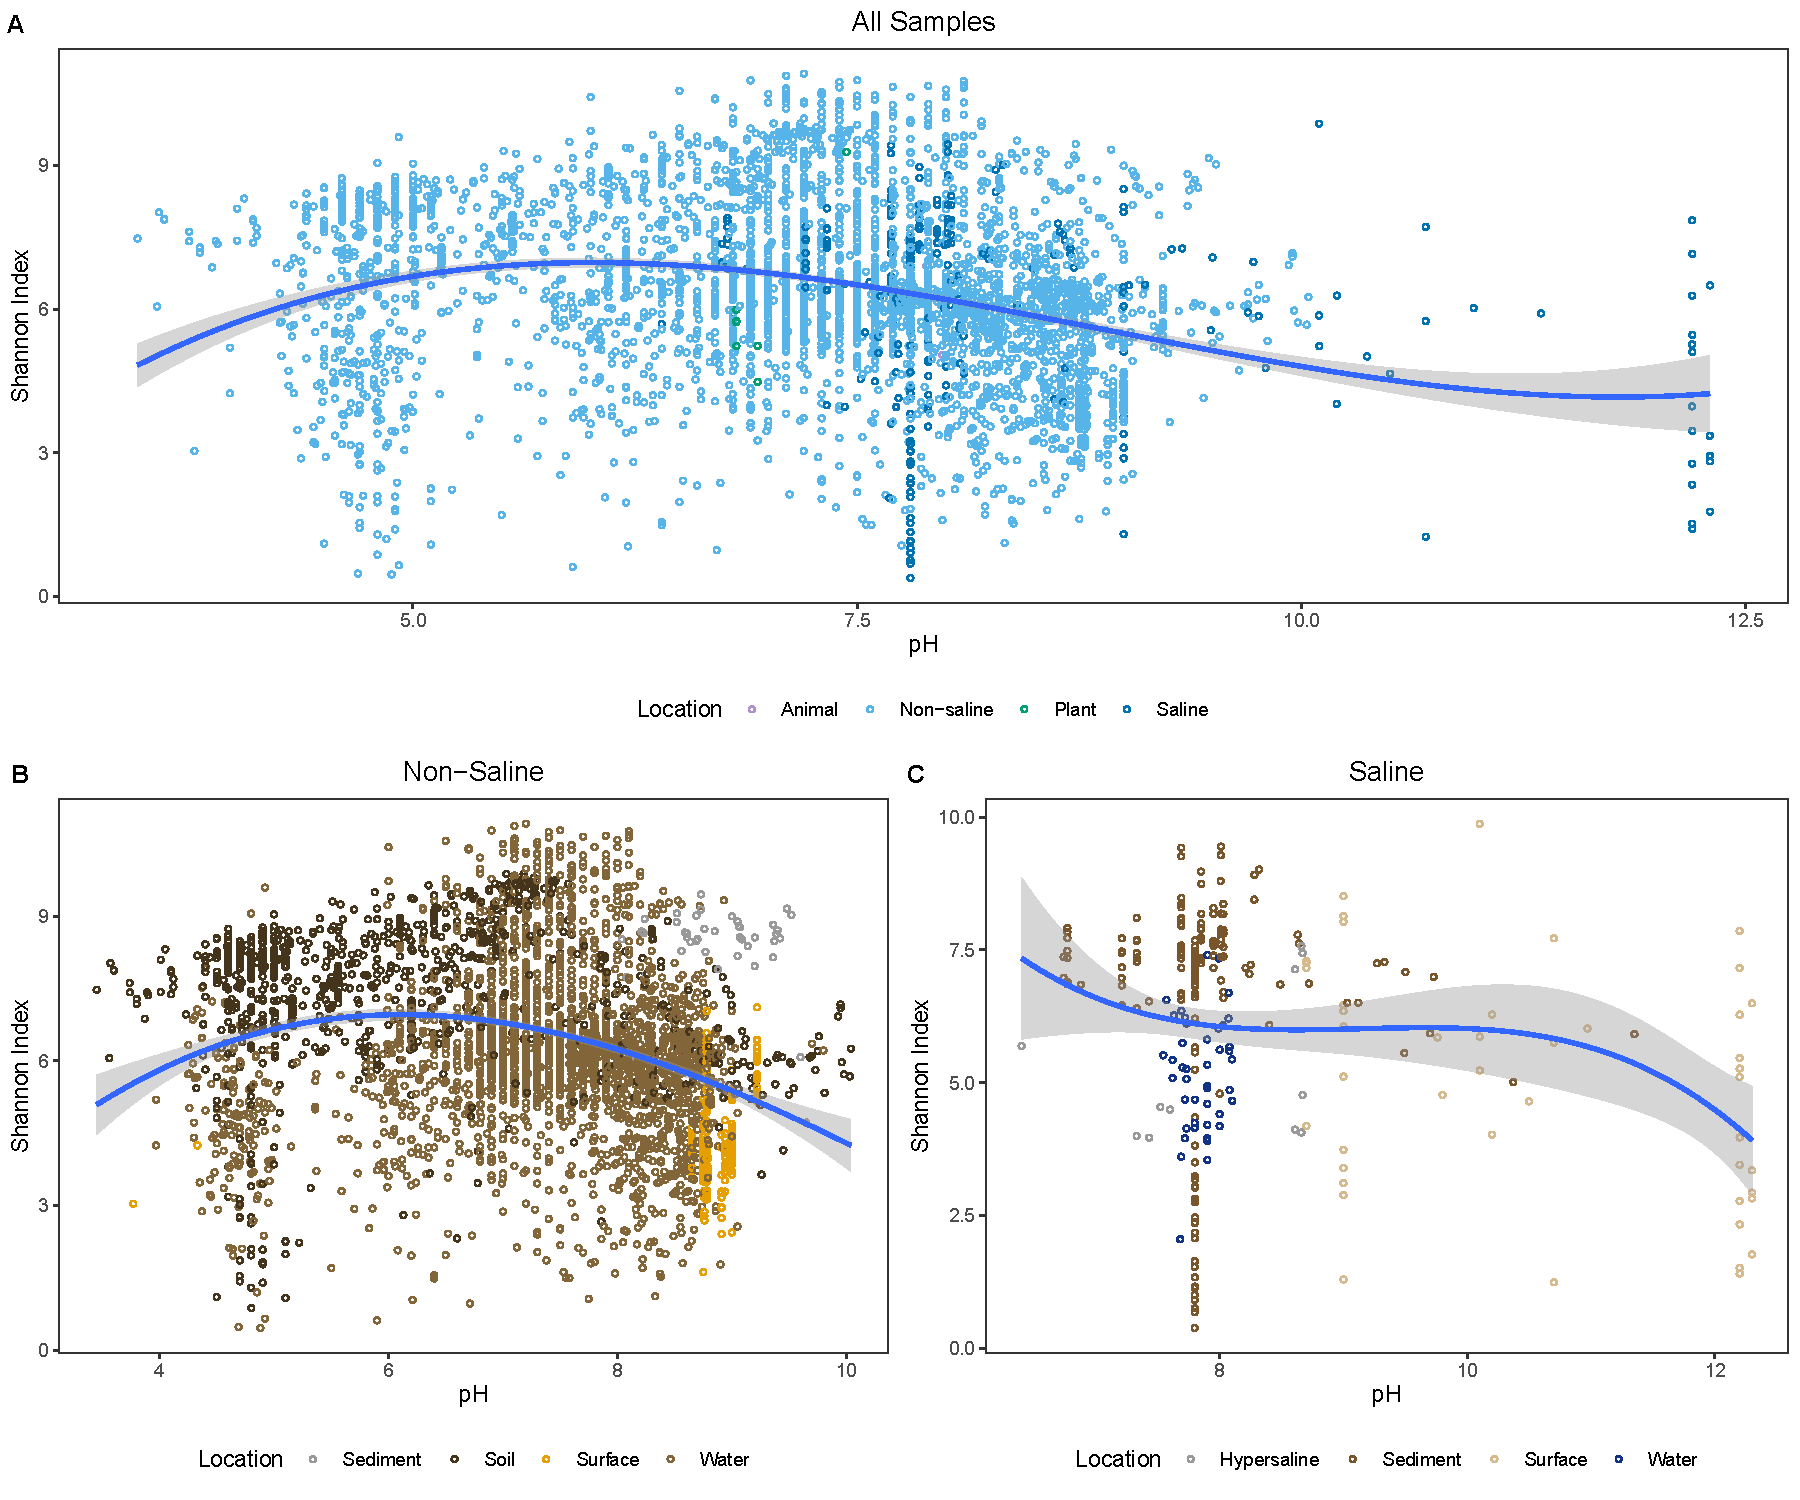
\includegraphics[scale=0.33]{./Figures/Shan_pH_empo2}
    \caption{\textbf{The relationship between Shannon index and pH.} A: Trend of Shannon index with pH for samples in the whole dataset. B: Trend of Shannon index with pH for non-saline samples. C: Trend of Shannon index with pH for saline samples.}
    \label{fig:Shan_pH}
\end{figure}

\begin{figure}[H]
    \centering
    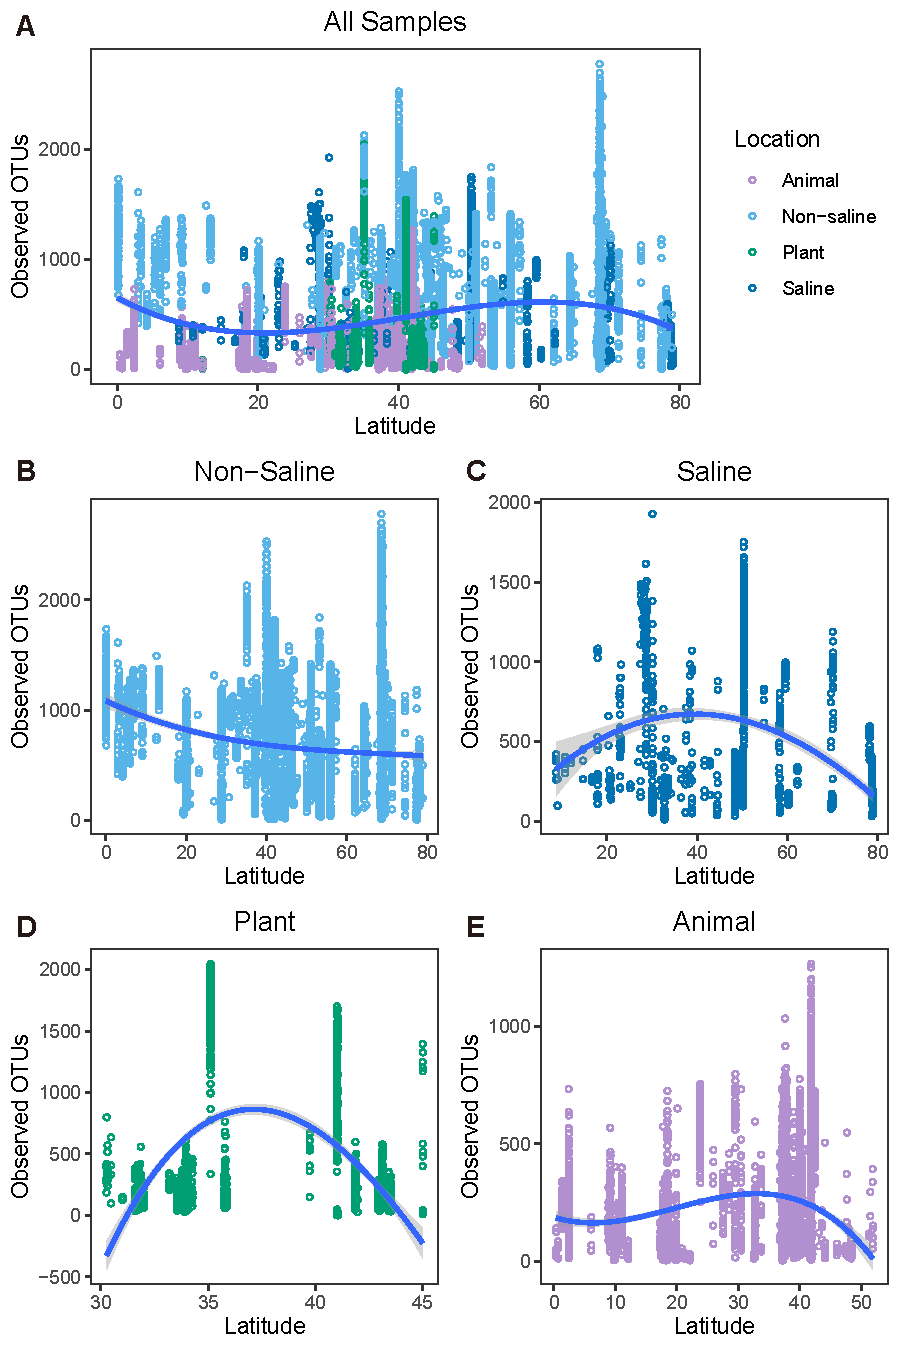
\includegraphics[scale=0.33]{./Figures/OO_lati_empo2}
    \caption{\textbf{The relationship between observed OTUs and latitude.} A: Trend of observed OTUs with latitude for samples in the whole dataset. B: Trend of observed OTUs with latitude for non-saline samples. C: Trend of observed OTUs with latitude for saline samples. D: Trend of observed OTUs with latitude for plant samples. E: Trend of observed OTUs with latitude for animal samples.}
    \label{fig:OO_lati}
\end{figure}

\begin{figure}[H]
    \centering
    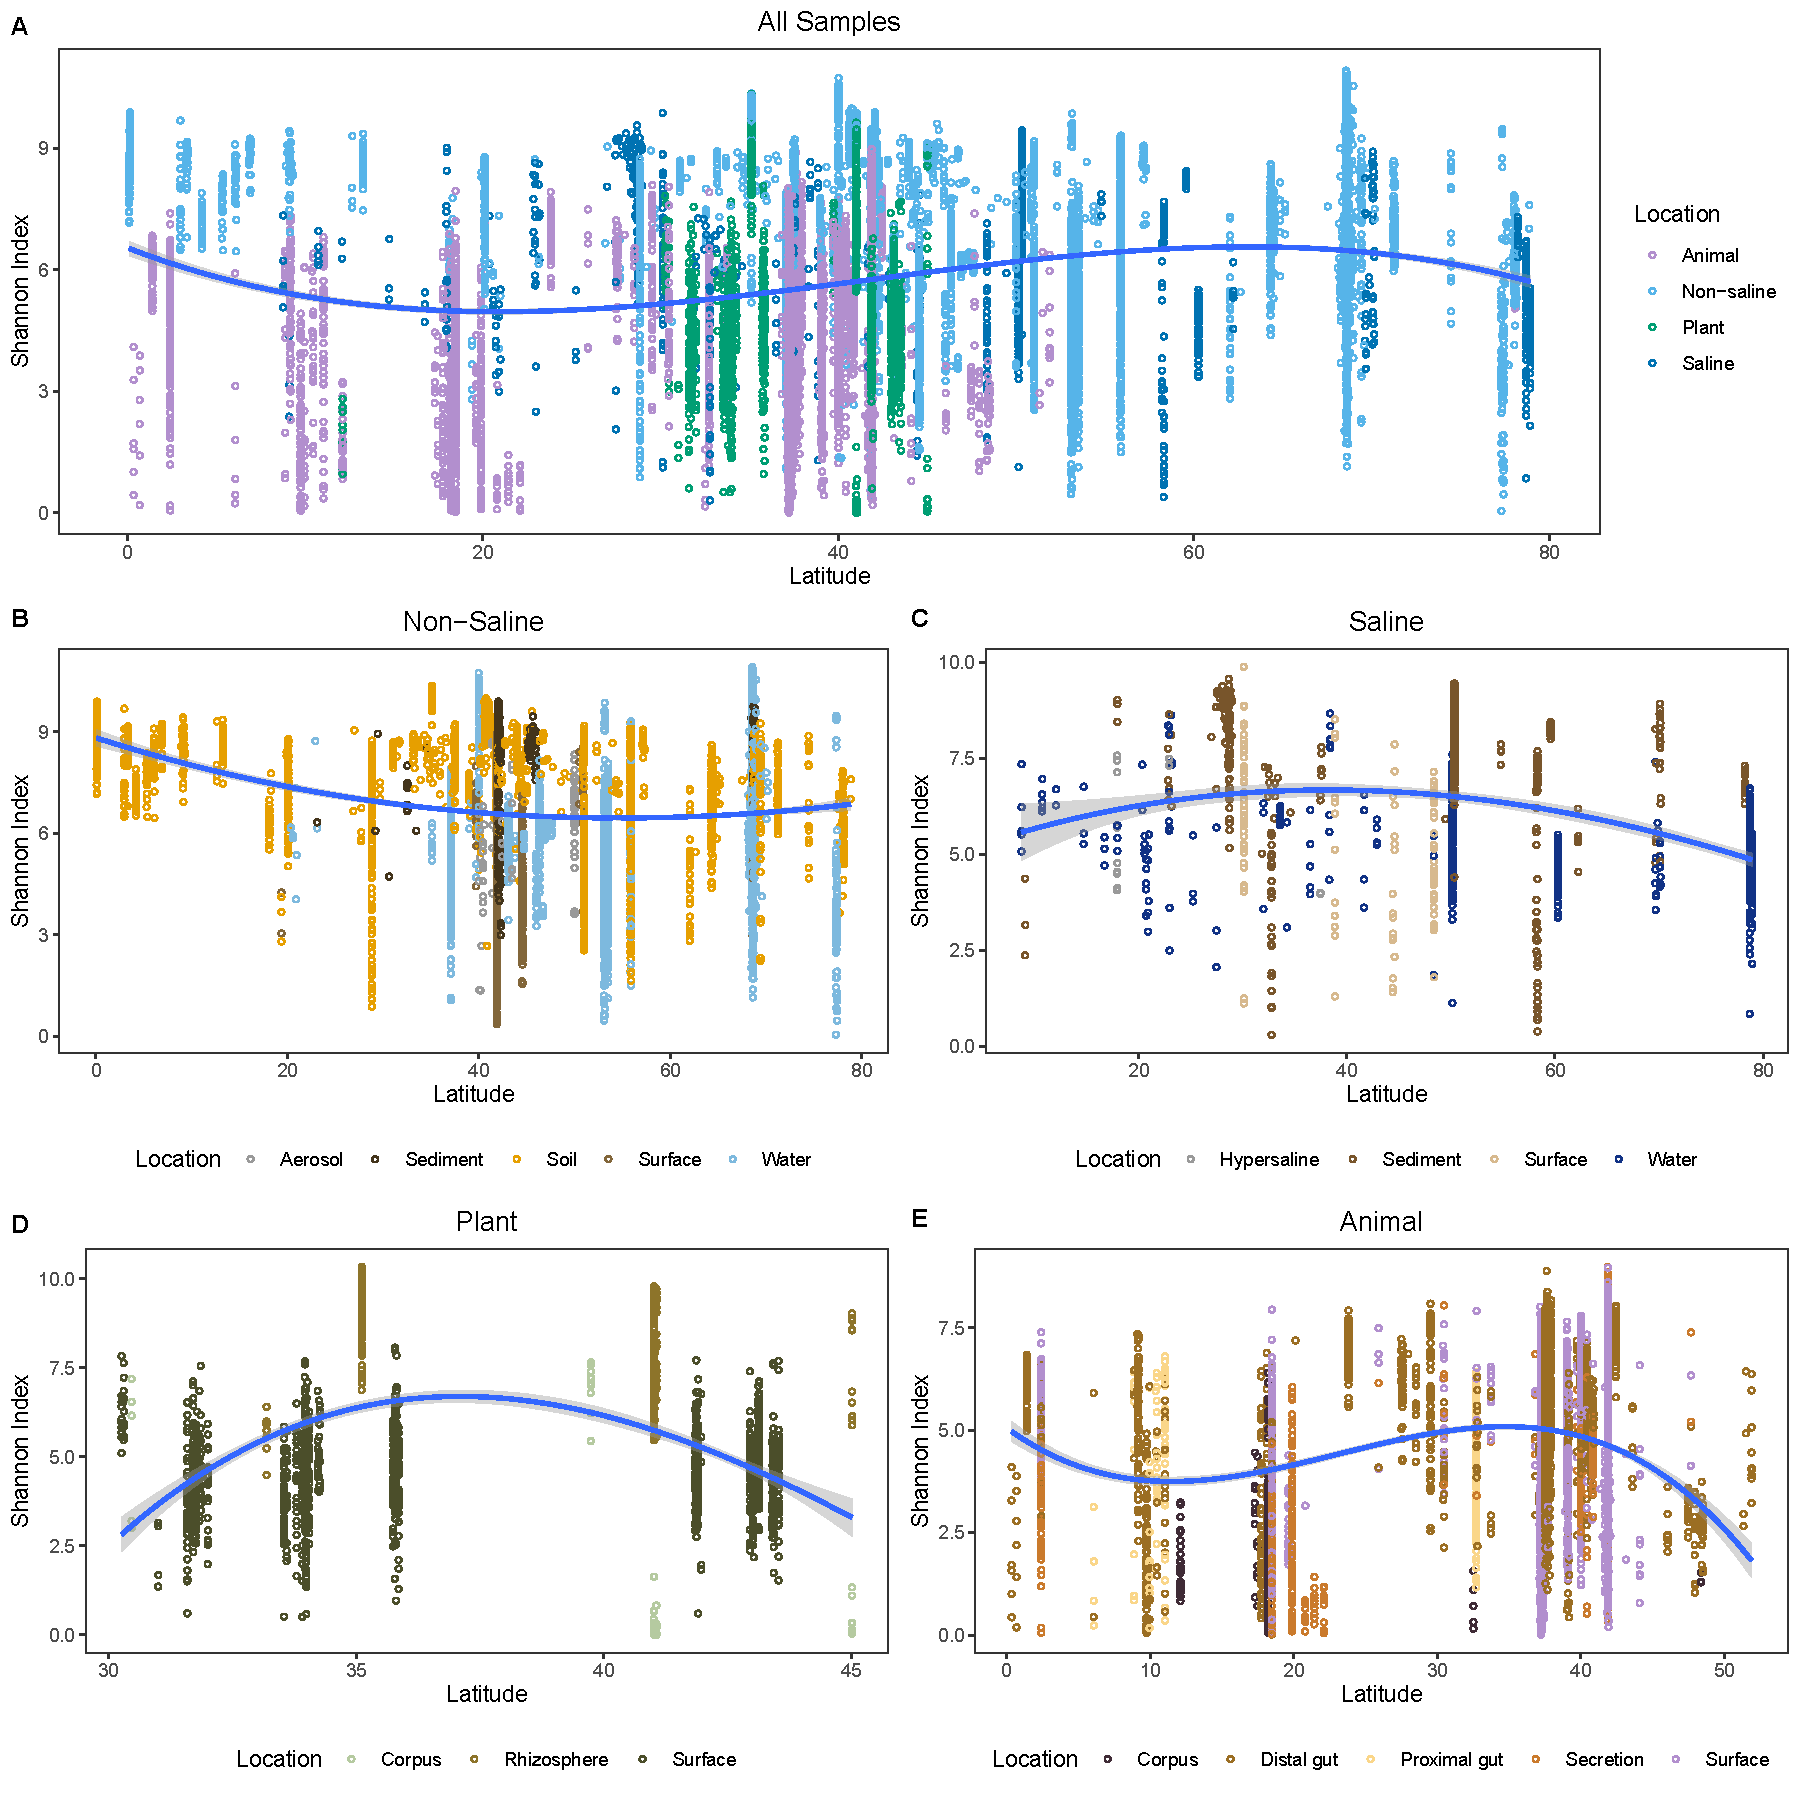
\includegraphics[scale=0.33]{./Figures/Shan_lati_empo2}
    \caption{\textbf{The relationship between Shannon index and latitude.} A: Trend of Shannon index with latitude for samples in the whole dataset. B: Trend of Shannon index with latitude for non-saline samples. C: Trend of Shannon index with latitude for saline samples. D: Trend of Shannon index with latitude for plant samples. E: Trend of Shannon index with latitude for animal samples.}
    \label{fig:Shan_lati}
\end{figure}

\begin{figure}[H]
    \centering
    \includegraphics[scale=0.33]{./Figures/OO_lati_empo3}
    \caption{\textbf{The relationship between observed OTUs and latitude.} A: Trend of observed OTUs with latitude for soil samples. B: Trend of observed OTUs with latitude for non-saline water (water and sediment) samples. C: Trend of observed OTUs with latitude for saline water (water and sediment) samples. D: Trend of observed OTUs with latitude for non-saline sediment samples. E: Trend of observed OTUs with latitude for non-saline surface samples. F: Trend of observed OTUs with latitude for non-saline water samples. G: Trend of observed OTUs with latitude for saline sediment samples. H: Trend of observed OTUs with latitude for saline surface samples. I: Trend of observed OTUs with latitude for saline water samples. J: Trend of observed OTUs with latitude for animal surface samples. K: Trend of observed OTUs with latitude for plant surface samples. L: Trend of observed OTUs with latitude for plant rhizosphere samples.}
    \label{fig:OO_lati3}
\end{figure}


\begin{figure}[H]
    \centering
    \includegraphics[scale=0.33]{./Figures/Shan_lati_empo3}
    \caption{\textbf{The relationship between Shannon index and latitude.} A: Trend of Shannon index with latitude for soil samples. B: Trend of Shannon index with latitude for non-saline water (water and sediment) samples. C: Trend of Shannon index with latitude for saline water (water and sediment) samples. D: Trend of Shannon index with latitude for non-saline sediment samples. E: Trend of Shannon index with latitude for non-saline surface samples. F: Trend of Shannon index with latitude for non-saline water samples. G: Trend of Shannon index with latitude for saline sediment samples. H: Trend of Shannon index with latitude for saline surface samples. I: Trend of Shannon index with latitude for saline water samples. J: Trend of Shannon index with latitude for animal surface samples. K: Trend of Shannon index with latitude for plant surface samples. L: Trend of Shannon index with latitude for plant rhizosphere samples.}
    \label{fig:Shan_lati3}
\end{figure}


\subsection{The relationships between alpha diversity and environmental variables}

\begin{figure}[H]
    \centering
    \includegraphics[scale=0.15]{./Figures/PairsPlot}
    \caption{\textbf{The relationship between alpha diversity indices, temperature, pH and latitude.} A: The relationship between Chao1 index, temperature, pH and latitude. B: The relationship between observed OTUs, temperature, pH and latitude. C: The relationship between Shannon index, temperature, pH and latitude..}
    \label{fig:Pairs}
\end{figure}

\begin{figure}[H]
    \centering
    \includegraphics[scale=0.33]{./Figures/OO_LM_PM_simpleTpL}
    \caption{\textbf{Linear and polynomial regression models of Observed OTUs with a single environmental variable.} A: Linear model of Observed OTUs versus temperature. B: Linear model of Observed OTUs versus pH. C: Linear model of Observed OTUs versus latitude. D: Polynomial regression model of Observed OTUs versus temperature. E: Polynomial regression model of Observed OTUs versus pH. F: Polynomial regression model of Observed OTUs versus latitude.}
    \label{fig:OO_simpleTpL}
\end{figure}

\begin{figure}[H]
    \centering
    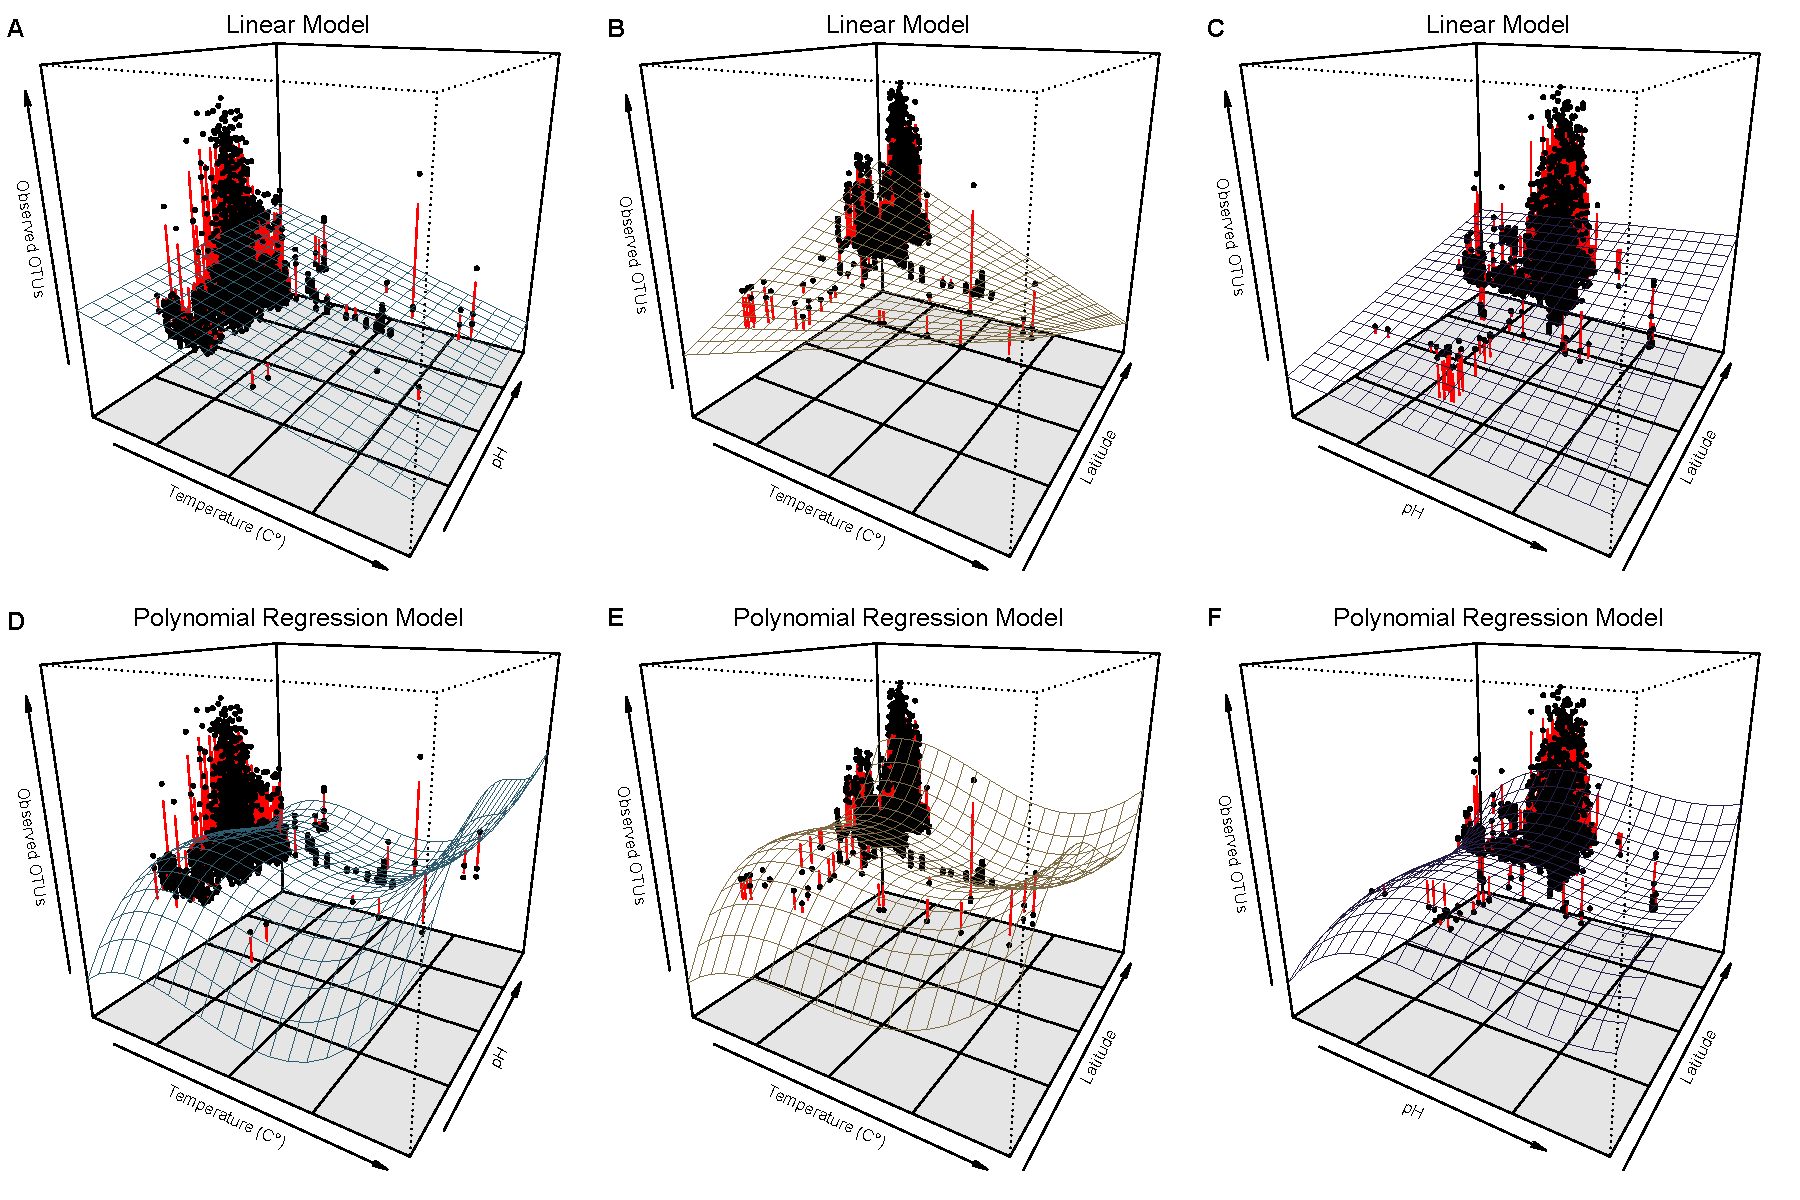
\includegraphics[scale=0.33]{./Figures/OO_LM_PM_all_2EVs_3D}
    \caption{\textbf{Linear and polynomial regression models of Observed OTUs with two environmental variables.} A: Linear model of Observed OTUs versus temperature and pH. B: Linear model of Observed OTUs versus temperature and latitude. C: Linear model of Observed OTUs versus pH and latitude. D: Polynomial regression model of Observed OTUs versus temperature and pH. E: Polynomial regression model of Observed OTUs versus temperature and latitude. F: Polynomial regression model of Observed OTUs versus pH and latitude.}
    \label{fig:OO_2EVs}
\end{figure}

\begin{figure}[H]
    \centering
    \includegraphics[scale=0.33]{./Figures/Shan_LM_PM_simpleTpL}
    \caption{\textbf{Linear and polynomial regression models of Shannon index with a single environmental variable.} A: Linear model of Shannon index versus temperature. B: Linear model of Shannon index versus pH. C: Linear model of Shannon index versus latitude. D: Polynomial regression model of Shannon index versus temperature. E: Polynomial regression model of Shannon index versus pH. F: Polynomial regression model of Shannon index versus latitude.}
    \label{fig:Shan_simpleTpL}
\end{figure}

\begin{figure}[H]
    \centering
    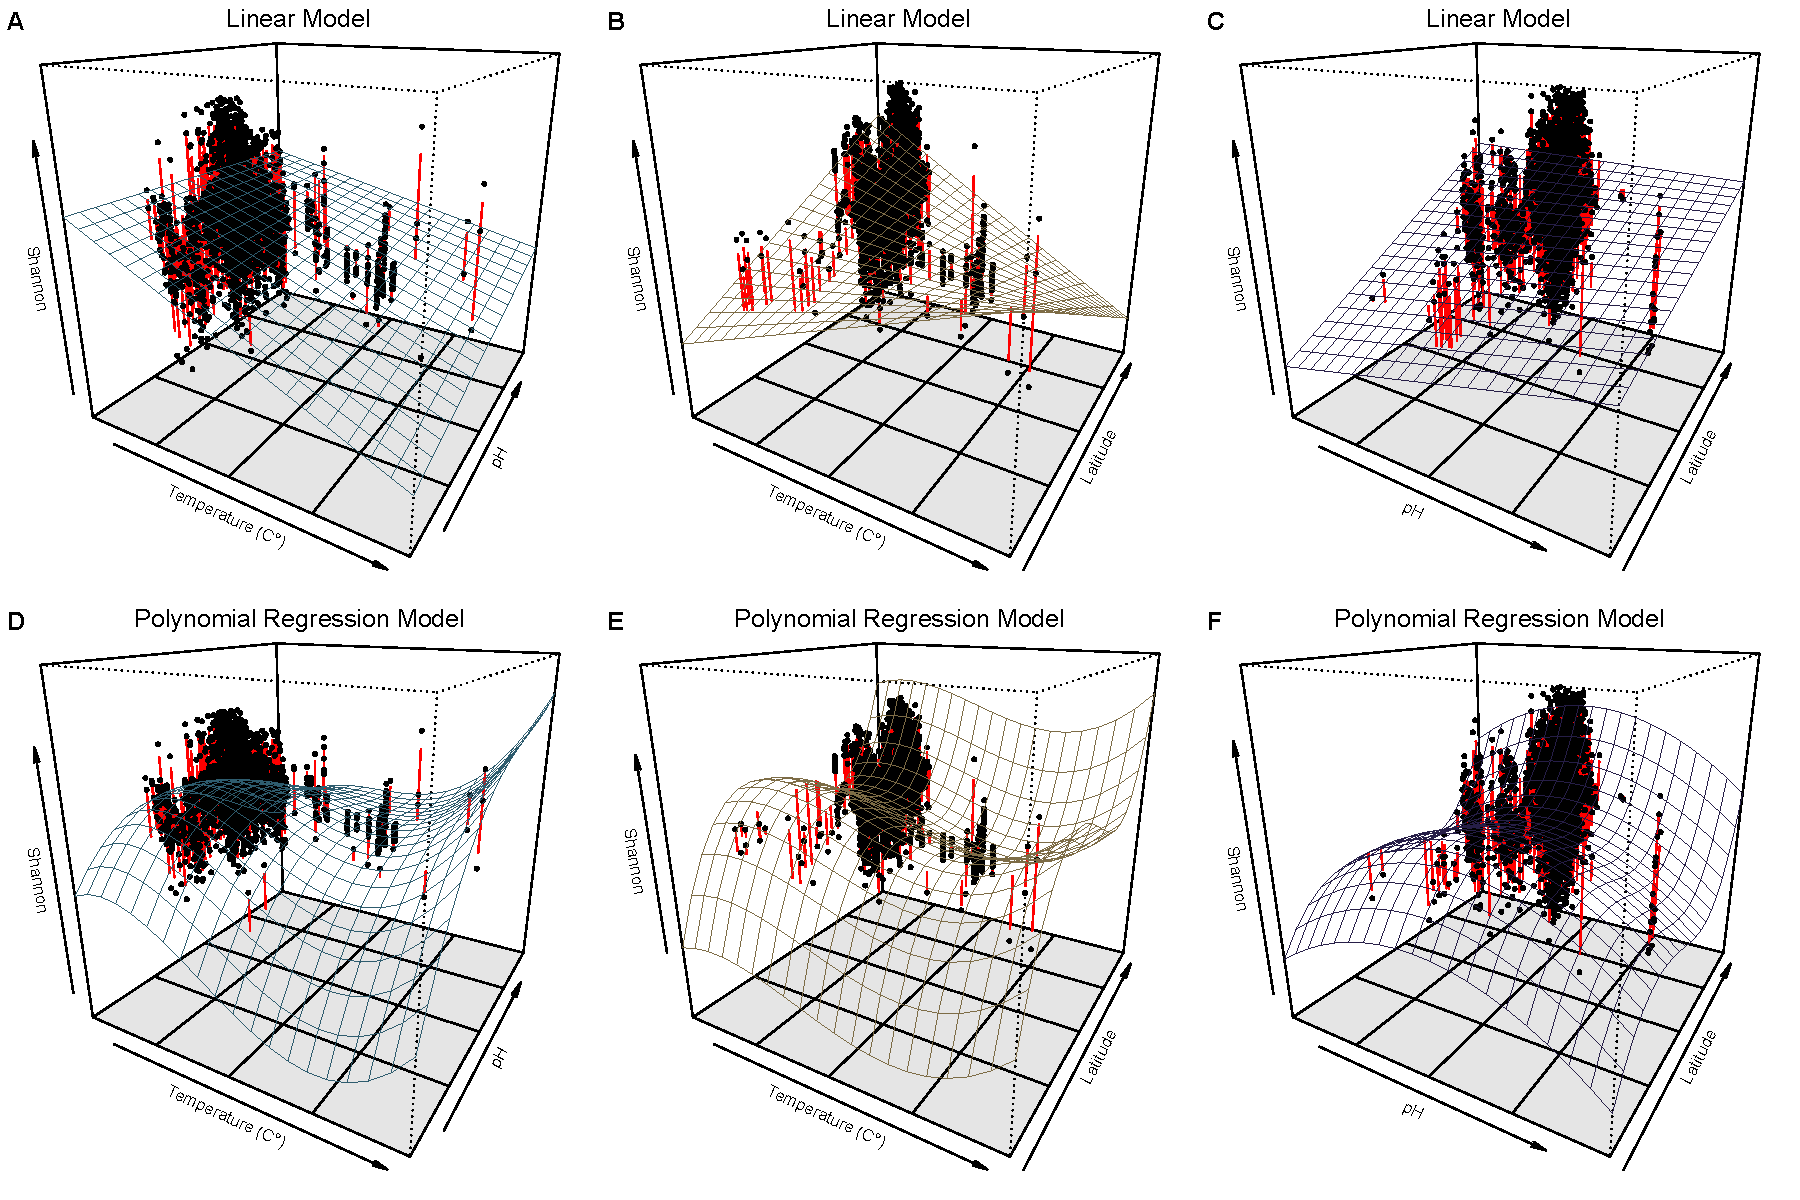
\includegraphics[scale=0.33]{./Figures/Shan_LM_PM_all_2EVs_3D}
    \caption{\textbf{Linear and polynomial regression models of Shannon index with two environmental variables.} A: Linear model of Shannon index versus temperature and pH. B: Linear model of Shannon index versus temperature and latitude. C: Linear model of Shannon index versus pH and latitude. D: Polynomial regression model of Shannon index versus temperature and pH. E: Polynomial regression model of Shannon index versus temperature and latitude. F: Polynomial regression model of Shannon index versus pH and latitude.}
    \label{fig:Shan_2EVs}
\end{figure}

\begin{table}[H]
    \caption{R-square of the EMPO3 models between Chao1 index, observed OTUs and Shannon index and environmental variables.}
    \centering
    \begin{tabular}{ |m{1cm}<{\centering}|m{1.3cm}<{\centering}|m{1.3cm}<{\centering}|m{1.3cm}<{\centering}|m{1.3cm}<{\centering}|m{1.3cm}<{\centering}|m{1.3cm}<{\centering}|m{1.3cm}<{\centering}|m{1.3cm}<{\centering}|m{1.3cm}<{\centering}|} 
    \hline
     $R^{2}$ (NS-Water) & Chao1 (LM) & Chao1 (PM) & Chao1 (RF) & Shannon (LM) & Shannon (PM) & Shannon (RF) & OTUs (LM) & OTUs (PM) & OTUs (RF) \\
     \hline
    T*p*L & 0.1781 & 0.1957 & 0.3979 & 0.2236 & 0.2355 & 0.322 & 0.1665 & 0.1829 & 0.3909 \\
    T*p & NULL & 0.1027 & 0.14 & 0.01416 & 0.1145 & 0.1534 & NULL & 0.09218 & 0.1284 \\
    T*L & 0.1458 & 0.1663 & 0.4269 & 0.2064 & 0.2165 & 0.3233 & 0.1363 & 0.1544 & 0.4304 \\
    p*L & NULL & 0.1344 & 0.4308 & 0.1962 & 0.2064 & 0.3186 & NULL & 0.1233 & 0.4149 \\
    T & 0.003247 & 0.06321 & 0.0186 & 0.0103 & 0.0522 & NULL & 0.004906 & 0.05587 & 0.0116 \\
    p & NULL & 0.06568 & 0.0994 & 0.003669 & 0.09646 & 0.1128 & NULL & 0.06064 & 0.0837 \\
    L & 0.1295 & 0.1327 & 0.4653 & 0.1854 & 0.1961 & 0.3463 & 0.116 & 0.1206 & 0.4609 \\
    \hline
    \hline
     $R^{2}$ (NS-Surf) & Chao1 (LM) & Chao1 (PM) & Chao1 (RF) & Shannon (LM) & Shannon (PM) & Shannon (RF) & OTUs (LM) & OTUs (PM) & OTUs (RF) \\
     \hline
    T*p*L & 0.6096 & 0.6594 & 0.6567 & 0.4957 & 0.5505 & 0.4803 & 0.5749 & 0.6241 & 0.6213 \\
    T*p & 0.4078 & 0.4895 & 0.6621 & 0.273 & 0.2916 & 0.4764 & 0.3603 & 0.4297 & 0.6243 \\
    T*L & NULL & 0.6011 & 0.6373 & NULL & 0.4443 & 0.463 & NULL & 0.5543 & 0.5965 \\
    p*L & 0.2897 & 0.558 & 0.642 & 0.1716 & 0.393 & 0.4681 & 0.2448 & 0.5036 & 0.6008 \\
    T & 0.2403 & 0.4724 & 0.6525 & 0.1373 & 0.2693 & 0.4696 & 0.205 & 0.4216 & 0.6164 \\
    p & 0.038 & 0.3264 & 0.6354 & 0.03825 & 0.1939 & 0.4225 & 0.03848 & 0.276 & 0.5914 \\
    L & NULL & 0.285 & 0.2741 & NULL & 0.2714 & 0.2542 & NULL & 0.2773 & 0.2656 \\
    \hline
    \hline
     $R^{2}$ (S-Sedi) & Chao1 (LM) & Chao1 (PM) & Chao1 (RF) & Shannon (LM) & Shannon (PM) & Shannon (RF) & OTUs (LM) & OTUs (PM) & OTUs (RF) \\
     \hline
    T*p*L & 0.5044 & 0.5044 & 0.4741 & NULL & NULL & 0.4035 & 0.578 & 0.578 & 0.5295 \\
    T*p & NULL & 0.4832 & 0.4342 & NULL & NULL & 0.3925 & NULL & 0.5499 & 0.5121 \\
    T*L & NULL & 0.4758 & 0.4672 & NULL & NULL & 0.3988 & NULL & 0.5554 & 0.5355 \\
    p*L & 0.5016 & 0.5018 & 0.4709 & 0.4109 & NULL & 0.3988 & 0.5717 & 0.5795 & 0.5416 \\
    T & 0.01735 & 0.4322 & 0.4677 & NULL & 0.1402 & 0.3899 & 0.01459 & 0.5115 & 0.5303 \\
    p & NULL & 0.09837 & 0.4275 & NULL & 0.1067 & 0.3854 & NULL & 0.1161 & 0.4941 \\
    L & 0.449 & 0.4559 & 0.447 & 0.3903 & 0.4102 & 0.4007 & 0.5302 & 0.545 & 0.5301 \\
    \hline
    \end{tabular}    
    \label{tab:EMPO3models}
\end{table}

\begin{table}[H]
    \caption{R-square of the local samples models between Chao1 index, observed OTUs and Shannon index and environmental variables. Local 1, 2 and 3 are Yellowstone National Park, Großer Stechlinsee and Toolik Lake respectively.}
    \centering
    \begin{tabular}{ |m{1.3cm}<{\centering}|m{1.2cm}<{\centering}|m{1.2cm}<{\centering}|m{1.2cm}<{\centering}|m{1.4cm}<{\centering}|m{1.4cm}<{\centering}|m{1.4cm}<{\centering}|m{1.3cm}<{\centering}|m{1.3cm}<{\centering}|m{1.2cm}<{\centering}|} 
    \hline
     $R^{2}$ & Chao1 (LM) & Chao1 (PM) & Chao1 (RF) & Shannon (LM) & Shannon (PM) & Shannon (RF) & OTUs (LM) & OTUs (PM) & OTUs (RF) \\
     \hline
    Local 1 T*p & 0.4719 & 0.4918 & 0.6588 & 0.2912 & 0.3152 & 0.4806 & 0.412 & 0.433 & 0.6205 \\
    Local 2 T*p & NULL & NULL & NULL & 0.04069 & 0.04874 & NULL & 0.009332 & 0.0143 & NULL \\
    Local 3 T*p & 0.05701 & 0.08249 & 0.0461 & 0.04255 & 0.05284 & 0.0098 & 0.0594 & 0.08191 & 0.0555 \\
    Local 1 T & 0.2438 & 0.473 & 0.6529 & 0.1433 & 0.267 & 0.4715 & 0.2093 & 0.04204 & 0.6159 \\
    Local 2 T & NULL & 0.003542 & NULL & 0.009679 & 0.009679 & NULL & 0.001895 & 0.003983 & NULL \\
    Local 3 T & 0.01907 & 0.06512 & 0.0185 & 0.03076 & 0.04849 & NULL & 0.0247 & 0.0647 & 0.0272 \\
    Local 1 p & 0.2981 & 0.4996 & 0.6343 & 0.1678 & 0.289 & 0.4266 & 0.2529 & 0.4368 & 0.5872 \\
    Local 2 p & NULL & NULL & NULL & 0.03141 & 0.03629 & NULL & 0.007482 & 0.01022 & NULL \\
    Local 3 p & NULL & 0.00248 & NULL & NULL & NULL & NULL & NULL & 0.001819 & NULL \\
    \hline
    \end{tabular}    
    \label{tab:localmodels}
\end{table}

\end{document}

\end{spacing}
\end{document}